% !TEX root = ../OT4ML.tex

%%%%%%%%%%%%%%%%%%%%%%%%%%%%%%%%%%%%%%%%%%%%%%%%%%%%%%%%%%%%%%%%%%%%%%%%%%%
%%%%%%%%%%%%%%%%%%%%%%%%%%%%%%%%%%%%%%%%%%%%%%%%%%%%%%%%%%%%%%%%%%%%%%%%%%%
%%%%%%%%%%%%%%%%%%%%%%%%%%%%%%%%%%%%%%%%%%%%%%%%%%%%%%%%%%%%%%%%%%%%%%%%%%%
\chapter{Monge Problem between Measures}
\index{Monge!problem}% strictindex
\label{sec-monge}

The goal of this chapter is to pass from finite matching to transport between arbitrary probability laws. The central stakes are to define measures, push-forwards and Monge maps carefully enough that the discrete picture survives, while exposing why deterministic maps can fail to exist. Monge's original formulation~\cite{Monge1781} and modern treatments~\cite{Villani03,Villani09,SantambrogioBook,rachev1998mass} are the conceptual background for this transition.
\index{push-forward}% strictindex

The presentation of the previous chapter could only handle two sets with the same number of points. To relax this to a more general setting, one needs to consider probability distributions, so that the points are weighted by masses.

%%%%%%%%%%%%%%%%%%%%%%%%%%%%%%%%%%%%%%%%%%%%%%%%%%%%%%%%%%%%%%%%%%%%%%%%%%%
\section{Measures}
\label{sec-measures}

Measures are the language that lets point clouds, densities and singular objects be handled uniformly. We only recall the facts needed later: integration, total variation, densities and probabilistic laws.
\index{total variation}% strictindex

%%%
\paragraph{Histograms}
\index{histogram}% strictindex

The finite-dimensional model for a probability law is a nonnegative vector with unit total mass.

\begin{defn}[Probability simplex]\label{def-probability-simplex}
\index{probability simplex}% strictindex
\index{histogram}% strictindex
	The probability simplex of length $n$ is
	\[
		\simplex_n \eqdef \enscond{\a \in \RR_+^n}{ \sum_{i=1}^n \a_i = 1 }.
	\]
	Its elements are also called probability vectors or histograms.
\end{defn}

%%%
\paragraph{Discrete measure, empirical measure}
\index{discrete!measure}% strictindex
\index{empirical!measure}% strictindex

Probability vectors become measures once their masses are attached to locations.

\begin{defn}[Discrete measure]\label{def-discrete-measure}
\index{discrete!measure}% strictindex
\index{Dirac mass}% strictindex
	A discrete measure with weights $\a$ and locations $x_1,\dots,x_n\in\X$ is
	\eql{\label{eq-discr-meas}
			\al = \sum_{i=1}^n \a_i \de_{x_i},
	}
	where $\de_x$ is the Dirac mass at position $x$. It is a probability measure if $\a\in\simplex_n$, and a positive measure if all weights $\a_i$ are nonnegative.
\end{defn}
The Dirac mass should be thought of as a unit of mass infinitely concentrated at one location.
\index{probability measure}% strictindex
\index{Dirac mass}% strictindex
%
An ``empirical'' probability distribution is uniform on a point cloud, i.e. $\al=\frac{1}{n}\sum_i \de_{x_i}$.
%
In practice, in many applications, it is useful to be able to manipulate both the positions $x_i$ (``Lagrangian'' discretization) and the weights $\a_i$ (``Eulerian'' discretization). Lagrangian modification is usually more powerful (because it leads to adaptive discretization) but it breaks the convexity of most problems.


%%%%
\paragraph{General measures}

We consider Borel measures $\al \in \Mm(\X)$ on a metric space $(\Xx,d)$, meaning that $\al(A)$ is defined for every Borel set $A$ (obtained from open sets by countable unions, countable intersections and complements). Unless otherwise stated, the measures are finite.
\index{Borel set}% strictindex
\index{Borel measure}% strictindex
%
A Dirac measure $\de_x$ is then defined as $\de_x(A)=1$ if $x \in A$ and $0$ otherwise, and this extends by linearity for discrete measures of the form~\eqref{eq-discr-meas} as
\index{Dirac mass}% strictindex
\eq{
	\al(A) = \sum_{x_i \in A} \a_i
}
%
We denote $\Mm_+(\X)$ the subset of all positive measures on $\X$, i.e. $\al(A) \geq 0$ (and $\al(\X)<+\infty$ for the measure to be finite). The set of probability measures is denoted $\Mm_+^1(\X)$, which means that any $\al \in \Mm_+^1(\X)$ is positive, and that $\al(\X)=1$.
\index{probability measure}% strictindex

\paragraph{Polish metric spaces.}
Many measure-theoretic statements used later require a mild regularity assumption on the underlying space. The point is not to restrict applications, since Euclidean spaces, complete separable manifolds and separable Hilbert spaces are covered, but to exclude pathological measurable spaces where disintegration, tightness or weak convergence can fail to behave properly.
\index{metric space}% strictindex
\index{weak!convergence}% strictindex
\index{tightness}% strictindex

\begin{defn}[Polish metric space]\label{def-polish-metric-space}
\index{Polish space}% strictindex
	A metric space $(\X,d)$ is Polish if it is complete and separable: every Cauchy sequence converges in $\X$, and $\X$ contains a countable dense subset. More generally, a topological space is called Polish if its topology can be induced by some complete separable metric.
\index{complete metric space}% strictindex
\index{separable space}% strictindex
\index{countable dense subset}% strictindex
\end{defn}
Polish spaces are the natural ambient category for probability measures. Borel probability measures on them are regular, tightness gives compactness criteria, regular conditional probabilities and disintegrations exist under standard assumptions, and Wasserstein spaces remain Polish; see Proposition~\ref{prop-wasserstein-space-polish}.
\index{probability measure}% strictindex
\index{Borel measure}% strictindex
\index{conditional probability}% strictindex
\index{disintegration}% strictindex

\begin{defn}[Support of a measure]\label{def:support}
\index{support}% strictindex
	The support $\supp(\al)$ of a Borel measure $\al$ on a metric space $\Xx$ is the smallest closed set of full $\al$-mass. Equivalently, $x\in\supp(\al)$ if every open ball centered at $x$ has positive $\al$-mass.
\index{Borel measure}% strictindex
\end{defn}


%%%%
\paragraph{Radon measures}
\index{Radon!measure}% strictindex

Using Lebesgue integration, a Borel measure can be used to compute the integral of measurable functions (i.e. such that level sets $\enscond{x}{f(x) < t}$ are Borel sets), and we denote this pairing as
\index{Borel set}% strictindex
\index{measurable function}% strictindex
\index{Borel measure}% strictindex
\eq{
	\dotp{f}{\al} \eqdef \int f(x) \d\al(x).
}
Integration of such a measurable $f$ against a discrete measure $\al$ computes a sum
\eq{
	\int_\X f(x) \d\al(x) = \sum_{i=1}^n \a_i f(x_i).
}


This applies in particular to continuous test functions, which are Borel measurable.
%
Integration against a finite measure on a compact space thus defines a continuous linear form $f \mapsto \int f \d\al$ on the Banach space of continuous functions $(\Cc(\Xx),\norm{\cdot}_\infty)$, indeed $|\int f \d\al| \leq \norm{f}_\infty |\al|(\Xx)$. On compact spaces, the converse is true: every continuous linear form on $\Cc(\Xx)$ is represented by integration against a finite signed Radon measure. This is the Riesz--Markov--Kakutani representation theorem~\cite{rudin1987realcomplex,bogachev2007measure}. It identifies $\Mm(\Xx)$ with the Banach dual of $\Cc(\Xx)$, and this duality pairing $\dotp{f}{\al}$ will be crucial for the convex duality arguments used later.
\index{Banach space}% strictindex
\index{Banach dual}% strictindex
\index{linear form}% strictindex
\index{finite measure}% strictindex
\index{Riesz-Markov-Kakutani theorem}% strictindex
\index{dual!pairing}% strictindex
\index{Radon!measure}% strictindex

%%%%%
\paragraph{Relative densities.}
\index{density!ratio}% strictindex

Many formulas below compare measures through densities with respect to a reference measure.

\begin{defn}[Relative density]\label{def-relative-density}
\index{Lebesgue measure}% strictindex
\index{reference!measure}% strictindex
\index{density!relative}% strictindex
	If $\al$ is absolutely continuous with respect to a reference measure $\lambda$, its relative density is the Radon--Nikodym derivative
	\[
		\density{\al}\eqdef\frac{\d\al}{\d\lambda},
		\qquad
		\d\al(x)=\density{\al}(x)\d\lambda(x).
	\]
	Equivalently, for all $h\in\Cc(\Xx)$,
	\[
		\int_{\Xx} h(x) \d\al(x) = \int_{\Xx} h(x) \density{\al}(x) \d\lambda(x).
	\]
\end{defn}
On $\RR^d$ the reference $\lambda$ is often Lebesgue measure $\d x$.

%%%%%
\paragraph{Total variation norm.}
\index{total variation}% strictindex

The norm inherited from the duality $\Mm(\Xx)=\Cc(\Xx)^*$ is the total variation norm. We use the notation
\index{total variation}% strictindex
\begin{defn}[Total variation]\label{defn-total-variation}
	For a finite signed Radon measure $\al$ on a compact space $\Xx$,
\index{Radon!measure}% strictindex
	\[
		\norm{\al}_{\TV}
		\eqdef
		\usup{f \in \Cc(\Xx)} \enscond{\dotp{f}{\al}}{\norm{f}_\infty \leq 1}.
	\]
\end{defn}
This formula is useful because it computes the norm of a measure as the operator norm of the corresponding linear form on $\Cc(\Xx)$.
\index{linear form}% strictindex
\index{operator norm}% strictindex

The same norm also has a direct measure-theoretic expression. The absolute value of a signed measure is
\index{signed!measure}% strictindex
\[
	|\al|(A)
	\eqdef
	\usup{A=\cup_i B_i} \sum_i |\al(B_i)|,
\]
where the supremum is over finite or countable measurable partitions of $A$. Thus, if $\al=\sum_i \a_i \de_{x_i}$ with distinct atoms, $|\al|=\sum_i |\a_i|\de_{x_i}$; if $\d\al(x)=\rho(x)\d\lambda(x)$, then $\d|\al|(x)=|\rho(x)|\d\lambda(x)$.

\begin{prop}[Dual and measure definitions of total variation]\label{prop-tv-dual-measure}
\index{total variation}% strictindex
	For a finite signed Radon measure $\al$ on a compact space $\Xx$,
\index{Radon!measure}% strictindex
	\[
		\norm{\al}_{\TV}=|\al|(\Xx).
	\]
	Consequently $(\Mm(\Xx),\norm{\cdot}_{\TV})$ is isometrically the Banach dual of $(\Cc(\Xx),\norm{\cdot}_\infty)$.
\index{Banach dual}% strictindex
\end{prop}
\begin{proof}
	The inequality $\norm{\al}_{\TV}\leq |\al|(\Xx)$ follows from
	\[
		\abs{\int f\,\d\al}\leq \int |f|\,\d|\al|\leq \norm{f}_\infty |\al|(\Xx).
	\]
	For the reverse inequality, write the Jordan decomposition $\al=\al^+-\al^-$, so that $|\al|=\al^++\al^-$. The measurable sign $s=\frac{\d\al}{\d|\al|}$ takes values in $\{-1,1\}$ outside a $|\al|$-null set and satisfies $\d\al=s\,\d|\al|$. By regularity of Radon measures on compact spaces, $s$ can be approximated in $L^1(|\al|)$ by continuous functions $f_k$ with $\norm{f_k}_\infty\leq1$. Hence $\int f_k\,\d\al\to\int s\,\d\al=|\al|(\Xx)$, which proves the equality. The final statement is the Riesz--Markov--Kakutani representation theorem with this norm.
\index{Riesz-Markov-Kakutani theorem}% strictindex
\index{Jordan decomposition}% strictindex
\index{Radon!measure}% strictindex
\end{proof}

For two absolutely continuous measures $\d\al=\rho_\al\d\lambda$ and $\d\be=\rho_\be\d\lambda$, this gives the concrete formula
\[
	\norm{\al-\be}_{\TV}
	=
	\int_\Xx |\rho_\al(x)-\rho_\be(x)|\,\d\lambda(x).
\]
For two discrete measures written on the same union of supports, $\al=\sum_k a_k\delta_{z_k}$ and $\be=\sum_k b_k\delta_{z_k}$, with missing coefficients set to zero,
\[
	\norm{\al-\be}_{\TV}
	=
	\sum_k |a_k-b_k|.
\]
%%%%%
\paragraph{Probabilistic interpretation.}
\index{probabilistic coupling}% strictindex

Radon probability measures represent the laws of random variables. A random variable with values in $\X$ is a measurable map $X:\Omega\to\X$ from an abstract probability space $(\Omega,\PP)$. Its law is the Radon probability measure $\al$ defined by
\index{random variable}% strictindex
\index{probability measure}% strictindex
\[
	\al(A)=\PP(\enscond{\omega\in\Omega}{X(\omega)\in A})
	\qquad\text{for Borel sets } A\subset \X .
\index{Borel set}% strictindex
\]
Integrals with respect to this law are expectations:
\[
	\int_\X f(x)\,\d\al(x)=\mathbb{E}[f(X)].
\]


%%%%%%%%%%%%%%%%%%%%%%%%%%%%%%%%%%%%%%%%%%%%%%%%%%%%%%%%%%%%%%%%%%%%%%%%%%%
\section{Push Forward}
\index{push-forward}% strictindex
\label{sec-push-forward}


Push-forwards encode how maps move mass. This short section is the bridge between deterministic maps and linear operations on measures.
\index{push-forward}% strictindex

For some continuous map $\T : \X \rightarrow \Y$, we define the pushforward operator $\T_\sharp : \Mm(\X) \rightarrow \Mm(\Y)$.
%
For a Dirac mass, one has $\T_\sharp \de_{x} = \de_{\T(x)}$, and this formula is extended to arbitrary measures by linearity. In some sense, moving from $\T$ to $\T_\sharp$ is a way to linearize any map at the price of moving from a (possibly) finite-dimensional space $\Xx$ to the infinite-dimensional space $\Mm(\Xx)$, and this idea is central to many convex relaxation methods, most notably Lasserre's relaxation.
\index{Dirac mass}% strictindex
%
For discrete measures~\eqref{eq-discr-meas}, the pushforward operation consists simply in moving the positions of all the points in the support of the measure
\index{support}% strictindex
\eq{
	\T_{\sharp} \al \eqdef \sum_i \a_i \de_{\T(x_i)}.
}
For more general measures, for instance for those with a density, the notion of push-forward plays a fundamental role in describing spatial modifications of probability measures. The formal definition reads as follows.
\index{probability measure}% strictindex
\index{push-forward}% strictindex

\begin{defn}[Push-forward]\label{defn-pushfwd}
For $\T : \X \rightarrow \Y$, the push forward measure $\be = \T_\sharp \al \in \Mm(\Y)$ of some $\al \in \Mm(\X)$ satisfies
\eql{\label{eq-push-fwd}
	\foralls h \in \Cc(\Y), \quad \int_\Y h(y) \d \be(y) = \int_\X h(\T(x)) \d\al(x).
}
Equivalently, for any measurable set $B \subset \Y$, one has
\eql{\label{eq-equiv-pushfwd}
	\be(B) = \al( \enscond{x \in \X}{\T(x) \in B} ).
}
Note that $\T_\sharp$ preserves positivity and total mass, so that if $\al \in \Mm_+^1(\X)$ then $\T_\sharp \al \in \Mm_+^1(\Y)$.
\end{defn}


\begin{rem}[Pullback and push-forward]\label{rem-pullback-pushforward}\label{rem-push-forward-pull-back}
\index{pullback}% strictindex
\index{push-forward}% strictindex
	If $\T:\X\to\Y$ is continuous, the pullback by $\T$ is the linear operator
	\[
		\T^\sharp:\Cc(\Y)\to\Cc(\X),
		\qquad
		\T^\sharp g=g\circ\T .
	\]
	The definition of the push-forward is exactly the dual relation between this pullback on functions and the action of $\T_\sharp$ on measures:
\index{pullback}% strictindex
\index{push-forward}% strictindex
	\[
		\int_\X \T^\sharp g(x)\d\mu(x)
		=
		\int_\Y g(y)\d(\T_\sharp\mu)(y).
	\]
	In pairing notation,
	\[
		\left\langle \T^\sharp g,\mu\right\rangle_{\Cc(\X),\Mm(\X)}
		=
		\left\langle g,\T_\sharp\mu\right\rangle_{\Cc(\Y),\Mm(\Y)}.
	\]
	Thus push-forward is the adjoint operation to pullback, with the direction reversed. The two arrows should not be confused: $\T_\sharp$ transports mass from $\X$ to $\Y$, whereas $\T^\sharp$ transports test functions from $\Y$ back to $\X$.
\index{push-forward}% strictindex
\end{rem}


%%%%%%%
\begin{prop}[Push-forward formula for densities]\label{prop-push-forward-densities}
\index{push-forward}% strictindex
\index{density!formula}% strictindex
	Let $\alpha$ and $\beta$ have densities $\density{\al}$ and $\density{\be}$ on open subsets of $\RR^\dims$. Assume that $\T$ is a $C^1$ diffeomorphism and that $\beta=\T_\sharp\alpha$. Then, for all $x$,
	\eql{\label{eq-pfwd-density}
			\density{\al}(x) = |\det(\T'(x))| \density{\be}(\T(x)).
	}
	Equivalently, for $y=\T(x)$,
	\[
		\rho_\beta(y)=\rho_\alpha(\T^{-1}y)\,
		\frac{1}{|\det(\T'(\T^{-1}y))|}.
	\]
\end{prop}

\begin{proof}
Explicitly doing the change of variable $y=\T(x)$, so that $\d y = |\det(\T'(x))| \d x$ in formula~\eqref{eq-push-fwd} for measures with densities $(\density{\al},\density{\be})$ on $\RR^\dims$, one has for all $h \in \Cc(\Yy)$
\begin{align*}
	\int_\Yy h(y)\rho_\be(y) \d y &= \int_\Yy h(y) \d \be(y) = \int_\Xx h(\T(x)) \d \al(x) = \int_\Xx h(\T(x)) \rho_\al(x) \d x \\
		&= \int_\Yy h(y) \rho_\al(\T^{-1}y) \frac{\d y}{|\det(\T'(\T^{-1} y))|},
\end{align*}
which shows that
\eq{
	\rho_\be(y) = \rho_\al(\T^{-1}y) \frac{1}{|\det(\T'(\T^{-1} y))|}.
}
Since $\T$ is a diffeomorphism, one obtains equivalently
\eq{
		\density{\al}(x) = |\det(\T'(x))| \density{\be}(\T(x))
}
where $\T'(x) \in \RR^{\dims \times \dims}$ is the Jacobian matrix of $\T$ (the matrix formed by taking the gradient of each coordinate of $\T$).
%
This implies, denoting $y=\T(x)$
\eq{
	|\det(\T'(x))| = \frac{ \density{\al}(x) }{ \density{\be}(y) }.
}
\end{proof}
%%%%%%%


\begin{rem}[Probabilistic interpretation]
\index{probabilistic coupling}% strictindex
The law, i.e. probability distribution, of a random variable $X$ is the push-forward of $\PP$ by $X$, namely $\al=X_\sharp\PP$.
\index{random variable}% strictindex
\index{push-forward}% strictindex
%
Applying another push-forward $\be = \T_\sharp\al$ for $\T : \X \rightarrow \Y$, following~\eqref{eq-push-fwd}, is equivalent to defining another random variable $Y=\T(X)$, namely $\omega \in \Om \mapsto \T(X(\omega)) \in \Y$. Thus $\be$ is the law of $Y$.
%
Drawing a random sample $y$ from $Y$ is thus simply achieved by computing $y=\T(x)$ where $x$ is drawn from $X$.
\end{rem}

%%%%%%%%%%%%%%%%%%%%%%%%%%%%%%%%%%%%%%%%%%%%%%%%%%%%%%%%%%%%%%%%%%%%%%%%%%%
\section{Monge's Formulation}
\index{Monge!problem}% strictindex
\label{sec-monge-formulation}
\label{sec-continuous-monge}

Monge's problem asks for a deterministic map transporting one law onto another while minimizing a prescribed cost. This is the original formulation introduced by Monge in his memoir on the ``d\'eblai et remblai'' problem~\cite{Monge1781}. It is geometrically direct, because every source point is assigned one destination, but it is also analytically fragile: the feasible set is non-convex, it can be empty, and a map cannot split mass. These limitations are precisely what motivate Kantorovich's relaxation in the next section.
\index{Kantorovich!relaxation}% strictindex
\index{Monge!problem}% strictindex

\paragraph{Monge problem.}

Given $\al\in\Mm_+^1(\Xx)$, $\be\in\Mm_+^1(\Yy)$ and a cost $c:\Xx\times\Yy\to\RR_+$, the Monge problem is
\index{Monge!problem}% strictindex
\eql{\label{eq-monge-continuous}
	\Monge_c(\al,\be)
	\eqdef
	\inf_{\T:\Xx\to\Yy}
	\enscond{\int_\Xx c(x,\T(x))\d\al(x)}{\T_\sharp\al=\be}.
}
The constraint $\T_\sharp\al=\be$ means that $\T$ pushes the mass of $\al$ onto $\be$ in the sense of Definition~\ref{defn-pushfwd}.

\begin{prop}[Empirical Monge maps and matchings]\label{prop-empirical-monge-matching}
\index{Monge!problem}% strictindex
\index{empirical!Monge map}% strictindex
	Assume that the source atoms $x_1,\ldots,x_n$ are distinct and that
	\[
		\al=\frac1n\sum_{i=1}^n\de_{x_i},
		\qquad
		\be=\frac1n\sum_{j=1}^n\de_{y_j}.
	\]
	If $\T_\sharp\al=\be$, then for each distinct target value $z$ in the support of $\be$, exactly $n\be(\{z\})$ source atoms are mapped to $z$. In particular, if the $y_j$ are distinct, then there exists a permutation $\sigma\in\Perm(n)$ such that $\T(x_i)=y_{\sigma(i)}$ for all $i$. Conversely, every such assignment of source atoms to target atoms with the correct masses defines a feasible Monge map on the support of $\al$, and in the distinct-target case
	\[
		\int_\Xx c(x,\T(x))\d\al(x)=\frac1n\sum_{i=1}^n c(x_i,y_{\sigma(i)}).
	\]
	If source locations are repeated, they should first be merged into atoms with larger masses; such atoms cannot be split by a Monge map.
\end{prop}
\begin{proof}
	Since $\T_\sharp\al=\be$, all images $\T(x_i)$ must belong to the support of $\be$; otherwise the push-forward would give positive mass to a point outside that support. For any target atom $z$,
\index{push-forward}% strictindex
	\[
		\be(\{z\})=\al(\T^{-1}(\{z\}))=\frac1n\#\enscond{i}{\T(x_i)=z}.
	\]
	This proves the counting statement. If all target atoms have mass $1/n$, each target receives exactly one source atom, which is a permutation. The converse and the cost identity follow by direct substitution.
\end{proof}

\begin{prop}[Existence of transport maps from atomless sources]\label{prop-existence-transport-map-atomless}
\index{transport map}% strictindex
\index{measure!atomless}% strictindex
	Let $\al$ and $\be$ be Borel probability measures on Polish spaces, and assume that $\al$ is atomless. Then there exists a measurable map $\T$ such that $\T_\sharp\al=\be$.
\index{probability measure}% strictindex
\index{Polish space}% strictindex
\end{prop}
\begin{proof}
	A standard measure-isomorphism theorem identifies the atomless probability space generated by $\al$ with Lebesgue measure on $[0,1]$, modulo null sets~\cite{bogachev2007measure}. It is therefore enough to construct a map from $[0,1]$ to the target law $\be$. Choose a Borel isomorphism $i$ from the support of $\be$ onto a Borel subset of $[0,1]$, set $\nu=i_\sharp\be$, and use the generalized inverse of the cumulative distribution function of $\nu$. This map sends Lebesgue measure on $[0,1]$ to $\nu$ and takes values in $i(\supp\be)$ almost surely. Composing with $i^{-1}$ and then with the source isomorphism gives a measurable transport map from $\al$ to $\be$.
\index{Lebesgue measure}% strictindex
\index{support}% strictindex
\index{transport map}% strictindex
\index{cumulative!distribution function}% strictindex
\index{generalized!inverse}% strictindex
\index{measure!isomorphism}% strictindex
\end{proof}

\begin{rem}[Feasibility versus optimality]
	An optimal map solving~\eqref{eq-monge-continuous} might fail to exist for two distinct reasons. First, the constraint set can be empty, for instance if $\al=\de_x$ and $\be$ is not a single Dirac mass. Proposition~\ref{prop-existence-transport-map-atomless} shows that non-atomicity of the source removes this feasibility obstruction. Second, even when feasible maps exist, the infimum may fail to be attained because the class of maps is not closed under weak limits.
\index{weak!limit}% strictindex
\index{Dirac mass}% strictindex
\end{rem}

\begin{example}[A splitting obstruction]\label{ex-splitting-obstruction}
\index{splitting obstruction}% strictindex
	A classical example, discussed for instance in~\cite{SantambrogioBook}, takes $\al$ uniform on a vertical segment and $\be$ equal to the average of the uniform measures on two parallel vertical segments placed symmetrically to the left and to the right. For the quadratic cost, the relaxed Kantorovich optimizer splits each source point into its two symmetric targets. A deterministic Monge map cannot split one point into two destinations, so minimizing sequences must oscillate between the two sides and the Monge problem has no optimizer.
\index{cost!quadratic}% strictindex
\index{Monge!problem}% strictindex
\end{example}

\begin{example}[Semi-discrete Monge maps]
\index{semi-discrete!Monge map}% strictindex
	The Monge formulation is not symmetric in $\al$ and $\be$. It makes sense, for instance, when $\al$ has a density with respect to Lebesgue measure and $\be$ is discrete. On $\Xx=\Yy=\RR^d$, let $\be=\sum_j b_j\delta_{y_j}$ be supported on $\{y_1,\ldots,y_m\}$. A map $\T$ such that $\T_\sharp\al=\be$ defines a segmentation of the space into cells
\index{Lebesgue measure}% strictindex
	\[
		C_j\eqdef \T^{-1}(y_j),
		\qquad
		\al(C_j)=b_j.
	\]
	This is the semi-discrete setting. Chapter~\ref{sec-semidiscr-w1} explains how the cells become Laguerre cells for prescribed masses and ordinary Voronoi cells when the masses are free. If one exchanges the roles of $\al$ and $\be$ so that $\al$ is discrete, then no valid $\T$ exists in general: it is not possible to push forward a discrete measure to a measure with density.
\index{Laguerre cell}% strictindex
\index{semi-discrete!OT}% strictindex
\index{push-forward}% strictindex
\index{Voronoi cell}% strictindex
\end{example}

Figure~\ref{fig:monge-color-transfer-rgb} shows a finite-dimensional instance of this deterministic viewpoint. The source and target measures are empirical color clouds in RGB space, and the map transports colors while leaving pixel positions fixed. Grayscale equalization is one-dimensional, but transferring a full color palette requires transporting empirical measures in a three-dimensional color space, for instance RGB or Lab. Early color-transfer methods used affine statistics or iterated one-dimensional projections~\cite{reinhard2001color,pitie2005n}; replacing these projections by a genuine three-dimensional OT map gives a more intrinsic way to match palettes while preserving their geometry~\cite{rabin-ssvm-11}.
\index{empirical!measure}% strictindex
\index{one-dimensional!projection}% strictindex

\begin{figure}[H]
\centering
\begin{tabular}{@{}ccccc@{}}
\small source & \small $t=1/3$ & \small $t=2/3$ & \small transported & \small target \\[-.15em]
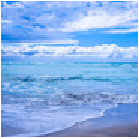
\includegraphics[width=.17\linewidth]{figures/monge-color-transfer-rgb--image-t000.pdf} &
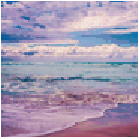
\includegraphics[width=.17\linewidth]{figures/monge-color-transfer-rgb--image-t033.pdf} &
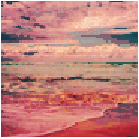
\includegraphics[width=.17\linewidth]{figures/monge-color-transfer-rgb--image-t067.pdf} &
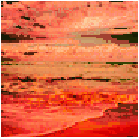
\includegraphics[width=.17\linewidth]{figures/monge-color-transfer-rgb--image-t100.pdf} &
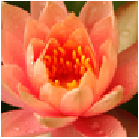
\includegraphics[width=.17\linewidth]{figures/monge-color-transfer-rgb--image-target.pdf} \\[-.1em]
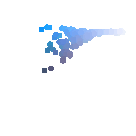
\includegraphics[width=.17\linewidth]{figures/monge-color-transfer-rgb--rgb-t000.pdf} &
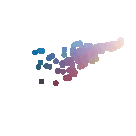
\includegraphics[width=.17\linewidth]{figures/monge-color-transfer-rgb--rgb-t033.pdf} &
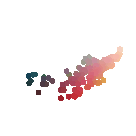
\includegraphics[width=.17\linewidth]{figures/monge-color-transfer-rgb--rgb-t067.pdf} &
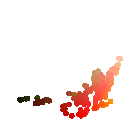
\includegraphics[width=.17\linewidth]{figures/monge-color-transfer-rgb--rgb-t100.pdf} &
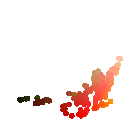
\includegraphics[width=.17\linewidth]{figures/monge-color-transfer-rgb--rgb-target.pdf}
\end{tabular}
\caption{Color transfer as a Monge map in RGB space, from a beach photograph to a flower photograph. The top row applies the palette map to the source image; the bottom row shows the empirical color clouds in the RGB cube. Only colors are transported here, not pixel locations.}
\label{fig:monge-color-transfer-rgb}
\end{figure}

\paragraph{Monge distance.}
\index{Monge!distance}% strictindex

When $\Xx=\Yy$ and $c(x,y)=d(x,y)^p$ for a metric $d$, set
\[
	\Ee_\al(\T)
	\eqdef
	\int_\Xx d(x,\T(x))^p\d\al(x).
\]
The Monge value defines the directed quantity
\eql{\label{eq-monge-distance}
\index{Monge!distance}% strictindex
	\tilde\Wass_p(\al,\be)^p
	\eqdef
	\inf_{\T:\Xx\to\Xx}
	\enscond{\Ee_\al(\T)}{\T_\sharp\al=\be}.
}
If the constraint set is empty, then $\tilde\Wass_p(\al,\be)=+\infty$.

\begin{prop}[Directed Monge distance]\label{prop-directed-monge-distance}
\index{Monge!distance}% strictindex
	Assume that $\Xx=\Yy$ is a metric space. The quantity $\tilde\Wass_p$ is nonnegative, vanishes only on the diagonal, and satisfies the triangle inequality. It is therefore a directed extended distance: it need not be symmetric and may take the value $+\infty$.
\index{triangle inequality}% strictindex
\end{prop}
\begin{proof}
	Nonnegativity is immediate. If $\tilde\Wass_p(\al,\be)=0$, choose feasible maps $\T_k$ with $\int d(x,\T_k(x))^p\d\al(x)\to0$. For every bounded $1$-Lipschitz function $h$,
\index{Lipschitz!function}% strictindex
	\[
		\left|\int h\d\be-\int h\d\al\right|
		=
		\left|\int h(\T_k(x))-h(x)\d\al(x)\right|
		\leq
		\left(\int d(x,\T_k(x))^p\d\al(x)\right)^{1/p}
		\longrightarrow0.
	\]
	Since bounded Lipschitz functions separate probability measures on metric spaces, $\al=\be$.
\index{probability measure}% strictindex
\index{Lipschitz!function}% strictindex

	We prove the triangle inequality. If $\tilde\Wass_p(\al,\be)=+\infty$ while both $\tilde\Wass_p(\al,\ga)$ and $\tilde\Wass_p(\ga,\be)$ were finite, there would be maps $S_\sharp\al=\ga$ and $T_\sharp\ga=\be$, hence $(T\circ S)_\sharp\al=\be$, a contradiction. Thus the inequality is automatic whenever the left-hand side is infinite. In the finite case, fix $\epsilon>0$ and choose $\epsilon$-minimizers $S_\sharp\al=\ga$ and $T_\sharp\ga=\be$ such that
\index{triangle inequality}% strictindex
	\[
		\Ee_\al(S)^{1/p}\leq\tilde\Wass_p(\al,\ga)+\epsilon,
		\qquad
		\Ee_\ga(T)^{1/p}\leq\tilde\Wass_p(\ga,\be)+\epsilon.
	\]
	The composed map is feasible from $\al$ to $\be$, and Minkowski's inequality gives
\index{Minkowski inequality}% strictindex
	\[
	\begin{aligned}
		\tilde\Wass_p(\al,\be)
		&\leq
		\left(\int d(x,T(S(x)))^p\d\al(x)\right)^{1/p} \\
		&\leq
		\left(\int d(x,S(x))^p\d\al(x)\right)^{1/p}
		+
		\left(\int d(S(x),T(S(x)))^p\d\al(x)\right)^{1/p} \\
		&=
		\Ee_\al(S)^{1/p}+\Ee_\ga(T)^{1/p}
		\leq
		\tilde\Wass_p(\al,\ga)+\tilde\Wass_p(\ga,\be)+2\epsilon.
	\end{aligned}
	\]
	Letting $\epsilon\to0$ gives the result.
\end{proof}

The directed value $\tilde\Wass_p$ is useful conceptually, but it is too rigid to be the main distance between measures: it can be infinite and asymmetric. The Kantorovich formulation remedies both issues by replacing maps with couplings.

%%%%%%%%%%%%%%%%%%%%%%%%%%%%%%%%%%%%%%%%%%%%%%%%%%%%%%%%%%%%%%%%%%%%%%%%%%%
\section{Existence and Uniqueness of the Monge Map}
\index{Monge!problem}% strictindex
\label{sec-monge-existence-uniqueness}

This section records the main regimes where Monge's deterministic formulation becomes well posed. Brenier's theorem is the central result: for the squared Euclidean cost, absolute continuity of the source restores existence, uniqueness and convex-potential structure.
\index{Brenier!theorem}% strictindex
\index{absolute continuity}% strictindex
\index{convex!potential}% strictindex

\paragraph{Brenier's theorem.}

Brenier's theorem~\cite{MR923203,Brenier91} ensures that, in $\RR^d$ for the quadratic cost, absolute continuity of the source is enough for Monge's problem to have a unique solution. It also gives the decisive structural description of this solution: the optimal map is not an arbitrary map, but the gradient of a convex potential.
\index{Brenier!theorem}% strictindex
\index{absolute continuity}% strictindex
\index{convex!potential}% strictindex
\index{cost!quadratic}% strictindex
\index{Monge!problem}% strictindex

\begin{thm}[Brenier]\label{thm-brenier}
	Let $\al,\be\in\Mm_+^1(\RR^d)$ have finite second moments, and assume that $\al$ is absolutely continuous with respect to Lebesgue measure. For the quadratic cost $c(x,y)=\norm{x-y}^2$, there exists a convex function $\phi:\RR^d\to\RR\cup\{+\infty\}$ such that
\index{Lebesgue measure}% strictindex
\index{convex!function}% strictindex
	\[
		\T=\nabla\phi,
		\qquad
		\T_\sharp\al=\be,
	\]
	and $\T$ is the unique optimal Monge map $\al$-almost everywhere. The optimal Kantorovich plan is $(\Id,\T)_\sharp\al$.
\index{Monge!problem}% strictindex
\end{thm}
\begin{proof}
	The proof uses the Kantorovich relaxation and duality developed later in Chapter~\ref{sec-dual}. Kantorovich duality for the quadratic cost gives optimal potentials $(f,g)$ with equality $f(x)+g(y)=\norm{x-y}^2$ on the support of any optimal plan. After subtracting the harmless quadratic terms, this equality is equivalent to the Fenchel equality $\phi(x)+\phi^*(y)=\dotp{x}{y}$ for a convex function $\phi$. Hence the support of every optimal plan lies in the graph of the subdifferential $\partial\phi$. Since $\al$ has a density and convex functions are differentiable Lebesgue-almost everywhere, $\partial\phi(x)$ is a singleton for $\al$-almost every $x$. The plan is therefore concentrated on the graph of $\T=\nabla\phi$, which proves that the relaxed optimizer is induced by a Monge map. Any two optimal plans are concentrated on the same single-valued graph $\al$-almost everywhere, which gives uniqueness of the map. This is the standard route behind Brenier's polar factorization theorem; related existence and uniqueness results for more general strictly convex costs are developed for instance in~\cite{gangbo1996geometry,caffarelli2002constructing,Villani09}.
\index{support}% strictindex
\index{subdifferential}% strictindex
\index{optimal plan}% strictindex
\index{Kantorovich!relaxation}% strictindex
\index{Kantorovich!duality}% strictindex
\index{polar factorization}% strictindex
\index{cost!quadratic}% strictindex
\end{proof}

\begin{defn}[Measures not charging hypersurfaces]\label{defn-not-charging-hypersurfaces}
\index{hypersurface}% strictindex
	A Borel measure $\al$ on $\RR^d$ does not charge hypersurfaces if $\al(S)=0$ for every countably $(d-1)$-rectifiable set $S$, i.e. every set that can be covered, up to an $\mathcal H^{d-1}$-null set, by countably many $C^1$ hypersurfaces.
\index{rectifiable set}% strictindex
\index{Hausdorff measure}% strictindex
\index{Borel measure}% strictindex
\end{defn}

\begin{rem}[A sharp source hypothesis]
\index{Brenier!source hypothesis}% strictindex
	The absolute-continuity assumption in Brenier's theorem can be weakened: for the quadratic cost, it is enough that $\al$ does not charge hypersurfaces~\cite{gangbo1996geometry,Villani09,SantambrogioBook}. The reason is that the set where a convex potential has a genuinely multi-valued subdifferential is contained in a countable union of lower-dimensional pieces. This condition is close to sharp. If the source gives positive mass to a segment or a hypersurface, the subdifferential may be multi-valued on a set of positive $\al$-mass, and the optimal relaxed plan may need to split mass, as in Example~\ref{ex-splitting-obstruction}.
\index{multi-valued subdifferential}% strictindex
\index{lower-dimensional set}% strictindex
\index{hypersurface}% strictindex
\index{subdifferential}% strictindex
\index{Brenier!theorem}% strictindex
\index{splitting obstruction}% strictindex
\index{absolute continuity}% strictindex
\index{convex!potential}% strictindex
\index{cost!quadratic}% strictindex
\end{rem}

\begin{rem}[Beyond the quadratic Euclidean cost]
\index{cost!quadratic}% strictindex
	Brenier's theorem is the cleanest statement because the squared Euclidean cost turns optimal maps into gradients of convex functions. For costs $c(x,y)=\norm{x-y}^p$ with $p>1$, or more generally costs $c(x,y)=h(x-y)$ with $h$ smooth and strictly convex, the same strategy gives a unique optimal map under absolute continuity of the source, but the map is written in terms of a $c$-convex potential. On a Riemannian manifold, the local analogue for the cost $d_M(x,y)^2/2$ uses the exponential map
\index{convex!function}% strictindex
\index{Brenier!theorem}% strictindex
\index{absolute continuity}% strictindex
\index{convex!potential}% strictindex
	\[
		\T(x)=\exp_x(-\nabla\phi(x)),
	\]
	where $\phi$ is $c$-convex. The main additional issues are the cut locus and regularity of geodesics, which is why the Euclidean statement is usually presented first. These extensions are part of McCann's displacement convexity theory and the general theory of optimal maps on manifolds~\cite{mccann1997convexity,Villani09}.
\index{displacement!convexity}% strictindex
\end{rem}

Brenier's theorem should be understood through the analogy between convex gradients and increasing functions. The gradient of a convex function is a monotone field:
\index{convex!function}% strictindex
\index{Brenier!theorem}% strictindex
\[
	\dotp{\nabla\phi(x)-\nabla\phi(x')}{x-x'}\geq0.
\]

\begin{rem}[Monotone fields need not be gradients]
\index{monotone!field}% strictindex
\index{gradient!field}% strictindex
	In dimensions larger than one, not all monotone fields are gradients of convex functions. Consider in $\RR^2$ the rotation matrix
\index{convex!function}% strictindex
	\[
		R_\theta=\begin{pmatrix}
		\cos\theta & -\sin\theta\\
		\sin\theta & \cos\theta
		\end{pmatrix}.
	\]
	The linear map $x\mapsto R_\theta x$ is monotone as soon as $|\theta|\leq\pi/2$, because
	\[
		\dotp{R_\theta x-R_\theta x'}{x-x'}
		=
		\dotp{R_\theta(x-x')}{x-x'}
		=
		\cos(\theta)\norm{x-x'}^2\geq0.
	\]
	However, for $\theta\neq0$, $R_\theta$ is not symmetric and therefore cannot be the gradient of a scalar potential. Indeed, if a linear field $Ax$ equals $\nabla\phi(x)$, then its Jacobian $A$ must be symmetric; equivalently, a quadratic potential $\phi(x)=\dotp{Bx}{x}/2$ has gradient $((B+B^\top)/2)x$. Thus monotonicity is weaker than Brenier optimality in dimension $d\geq2$.
\index{quadratic!potential}% strictindex
\end{rem}

\paragraph{Polar factorization.}
\index{polar factorization}% strictindex

Brenier's theorem does more than solve one transport problem: it provides a canonical way to extract the ``monotone part'' of an arbitrary map. Suppose one starts from a square-integrable deformation $u:\Omega\to\RR^d$, for instance a velocity snapshot, an image deformation or a generative map. The law $\nu=u_\sharp\lambda$ records where the mass ends up, but it forgets how the points of $\Omega$ were labelled before being sent there. Brenier's polar factorization~\cite{MR923203,Brenier91} separates these two effects. The map first applies a measure-preserving rearrangement $s$ of the source, which changes labels but not mass, and then applies the unique convex-gradient map $\nabla\phi$ sending the uniform source to the output law. Thus the Brenier factor is the canonical optimal-transport representative among all maps with the same image distribution. This is useful because it isolates the part of a map that carries genuine Wasserstein displacement from the volume-preserving noise of a parametrization. It is also a bridge to fluid mechanics, where measure-preserving maps describe incompressible relabellings, and to data analysis, where one often wants to compare maps modulo such relabellings.
\index{measure-preserving!map}% strictindex
\index{Brenier!theorem}% strictindex
\index{Brenier!factor}% strictindex

\begin{prop}[Polar factorization]\label{prop-polar-factorization}
\index{polar factorization}% strictindex
	Let $\Omega\subset\RR^d$ be endowed with normalized Lebesgue measure $\lambda$, and let $u\in L^2(\Omega;\RR^d)$. Assume that the law $\nu=u_\sharp\lambda$ has finite second moment. Then there exist a measure-preserving map $s:\Omega\to\Omega$ and a convex function $\phi$ such that
\index{Lebesgue measure}% strictindex
\index{convex!function}% strictindex
	\[
		u=\nabla\phi\circ s
		\qquad \lambda\text{-a.e.}
	\]
	The Brenier factor $\nabla\phi$ is unique $\lambda$-almost everywhere.
\index{Brenier!factor}% strictindex
\end{prop}
\begin{proof}
	By Brenier's theorem there is a unique gradient of a convex function $\T=\nabla\phi$ transporting $\lambda$ to $\nu$. The maps $u$ and $\T$ have the same image law. The rearrangement theorem for non-atomic probability spaces gives a measure-preserving map $s$ such that $u=\T\circ s$; equivalently, $s$ chooses, with the correct conditional probabilities, preimages of $u(x)$ under $\T$. Uniqueness of the Brenier factor follows from Theorem~\ref{thm-brenier}.
\index{non-atomic probability space}% strictindex
\index{conditional probability}% strictindex
\index{measure-preserving!map}% strictindex
\index{Brenier!theorem}% strictindex
\end{proof}

The name is meant to echo the usual polar decomposition of matrices. This analogy becomes literal for linear maps under the Gaussian reference measure. If $X\sim\Gaussian(0,\Id)$ and $u(x)=Ax$, then $u_\sharp\Gaussian(0,\Id)=\Gaussian(0,AA^\top)$. The Brenier map from $\Gaussian(0,\Id)$ to this Gaussian is $x\mapsto Sx$, where $S=(AA^\top)^{1/2}$ is symmetric positive semidefinite. Hence the decomposition $u=\nabla\phi\circ s$ reads
\index{matrix!polar decomposition}% strictindex
\index{reference!measure}% strictindex
\index{Brenier!map}% strictindex
\[
	A = S O,
	\qquad
	O=S^\dagger A,
\]
with $O$ orthogonal when $A$ is invertible, or a partial isometry in the singular case. The factor $Sx$ is the convex-gradient transport part, while $Ox$ preserves the standard Gaussian law. This finite-dimensional picture is often the fastest way to remember the general theorem: polar factorization is matrix polar decomposition with matrices replaced by maps and orthogonal transformations replaced by measure-preserving rearrangements.
\index{matrix!polar decomposition}% strictindex
\index{polar factorization}% strictindex

\paragraph{Displacement interpolation.}
\index{displacement!interpolation}% strictindex
\label{sec-monge-interpolation}

An optimal map does not only match two endpoint measures; it also tells how to draw a path between them. The construction is Lagrangian and geometric: each particle keeps its identity and travels at constant speed from its initial position to its image under the transport map.
\index{transport map}% strictindex

\begin{defn}[Monge and McCann displacement interpolation]\label{def-monge-mccann-interpolation}
\index{Monge!interpolation}% strictindex
\index{displacement!interpolation}% strictindex
	If $\T_\sharp\al=\be$, the Monge interpolation generated by $\T$ is the curve
	\[
		\T_t(x)\eqdef(1-t)x+t\T(x),
		\qquad
		\al_t\eqdef(\T_t)_\sharp\al,
		\qquad t\in[0,1].
	\]
	For the quadratic cost, when $\T$ is the optimal Brenier map, this curve is called McCann's displacement interpolation.
\end{defn}
McCann's displacement convexity theory~\cite{mccann1997convexity} clarifies the geometric meaning of interpolating along Brenier maps; this is the language of Wasserstein geodesics used later for barycenters in Section~\ref{sec-barycenters} and for gradient flows in Chapter~\ref{sec-wasserstein-gradient-flows}. If no Monge map exists, or if the optimal object splits mass, the same straight-line idea is applied to each active pair of a coupling, as explained in the Kantorovich interpolation of Section~\ref{sec-kantorovich-plan-interpolation}. The following proposition makes the constant-speed property precise for the directed Monge value.
\index{Brenier!map}% strictindex
\index{Monge!problem}% strictindex
\index{Wasserstein!geodesic}% strictindex
\index{gradient!flow}% strictindex
\index{Wasserstein!gradient flow}% strictindex
\index{displacement!interpolation}% strictindex
\index{Kantorovich!interpolation}% strictindex
\index{displacement!convexity}% strictindex
\index{Monge!interpolation}% strictindex
\index{cost!quadratic}% strictindex

\begin{prop}[Directed Monge displacement geodesics]\label{prop-monge-displacement-geodesic}
\index{Monge!geodesic}% strictindex
	Let $p\geq1$, let $\al,\be\in\Mm_+^1(\RR^d)$ have finite $p$-th moments, and let $\T$ be an optimal map for $\tilde\Wass_p(\al,\be)$ in~\eqref{eq-monge-distance}. Set $\al_t=(\T_t)_\sharp\al$ with $\T_t=(1-t)\Id+t\T$. Assume that, for every $t<1$, $\T_t$ is one-to-one on a full $\al$-measure Borel set, so that $\T_t^{-1}$ is defined $\al_t$-almost everywhere. Then, for $0\leq s\leq t\leq1$,
\index{Borel set}% strictindex
\index{Monge!distance}% strictindex
	\[
		\tilde\Wass_p(\al_s,\al_t)=(t-s)\tilde\Wass_p(\al,\be).
	\]
	Thus $t\mapsto\al_t$ is an oriented constant-speed geodesic for the directed Monge distance. In particular, for $p=2$, this applies to the Brenier map under the hypotheses of Theorem~\ref{thm-brenier}.
\index{constant-speed geodesic}% strictindex
\index{Monge!distance}% strictindex
\index{Brenier!map}% strictindex
\end{prop}
\begin{proof}
	The case $s=t$ is trivial, so assume $s<t$. Since $s<1$, the inverse $\T_s^{-1}$ is defined $\al_s$-almost everywhere along the transported particles. Define
	\[
		S_{s,t}\eqdef\T_t\circ\T_s^{-1}
		\qquad \al_s\text{-a.e.}
	\]
	Then $(S_{s,t})_\sharp\al_s=\al_t$, and, using the optimality of $\T$,
	\[
	\begin{aligned}
		\tilde\Wass_p(\al_s,\al_t)^p
		&\leq
		\int \norm{S_{s,t}(z)-z}^p\d\al_s(z) \\
		&=
		\int \norm{\T_t(x)-\T_s(x)}^p\d\al(x)
		=
		(t-s)^p\tilde\Wass_p(\al,\be)^p.
	\end{aligned}
	\]
	The same particle construction gives $\tilde\Wass_p(\al,\al_s)\leq s\tilde\Wass_p(\al,\be)$. If $t<1$, the map $\T\circ\T_t^{-1}$ sends $\al_t$ to $\be$ and gives $\tilde\Wass_p(\al_t,\be)\leq(1-t)\tilde\Wass_p(\al,\be)$; if $t=1$, this latter distance is zero. Using the triangle inequality from Proposition~\ref{prop-directed-monge-distance},
\index{triangle inequality}% strictindex
\index{Monge!distance}% strictindex
	\[
		\tilde\Wass_p(\al,\be)
		\leq
		\tilde\Wass_p(\al,\al_s)+\tilde\Wass_p(\al_s,\al_t)+\tilde\Wass_p(\al_t,\be)
		\leq
		s\tilde\Wass_p(\al,\be)+\tilde\Wass_p(\al_s,\al_t)+(1-t)\tilde\Wass_p(\al,\be).
	\]
	Hence $\tilde\Wass_p(\al_s,\al_t)\geq(t-s)\tilde\Wass_p(\al,\be)$, which proves equality. For a Brenier map $\T=\nabla\phi$, the map $\T_t$ is the gradient of
\index{Brenier!map}% strictindex
	\[
		x\mapsto (1-t)\frac{\norm{x}^2}{2}+t\phi(x),
	\]
	which is $(1-t)$-strongly convex for every $t<1$. On the full-measure set where $\phi$ is differentiable, this gives
	\[
		\dotp{\T_t(x)-\T_t(y)}{x-y}\geq(1-t)\norm{x-y}^2,
	\]
	so $\T_t$ is injective there. This gives the last claim.
\end{proof}

\begin{figure}[htbp]
\centering
\begin{tabular}{@{}ccccc@{}}
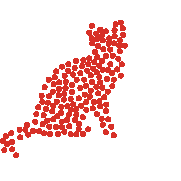
\includegraphics[width=.17\linewidth]{figures/monge-shape-mccann-interpolation--particles-t000.pdf} &
\index{McCann interpolation}% strictindex
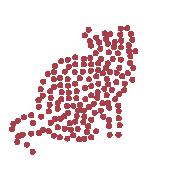
\includegraphics[width=.17\linewidth]{figures/monge-shape-mccann-interpolation--particles-t025.pdf} &
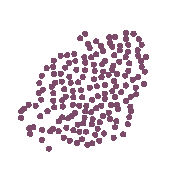
\includegraphics[width=.17\linewidth]{figures/monge-shape-mccann-interpolation--particles-t050.pdf} &
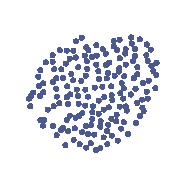
\includegraphics[width=.17\linewidth]{figures/monge-shape-mccann-interpolation--particles-t075.pdf} &
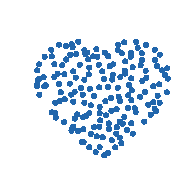
\includegraphics[width=.17\linewidth]{figures/monge-shape-mccann-interpolation--particles-t100.pdf} \\[-.1em]
\index{McCann interpolation}% strictindex
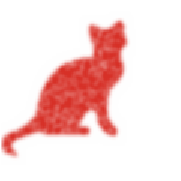
\includegraphics[width=.17\linewidth]{figures/monge-shape-mccann-interpolation--density-t000.pdf} &
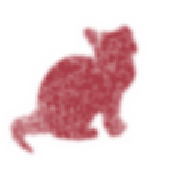
\includegraphics[width=.17\linewidth]{figures/monge-shape-mccann-interpolation--density-t025.pdf} &
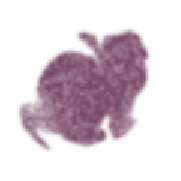
\includegraphics[width=.17\linewidth]{figures/monge-shape-mccann-interpolation--density-t050.pdf} &
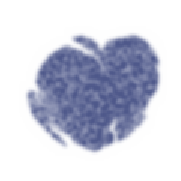
\includegraphics[width=.17\linewidth]{figures/monge-shape-mccann-interpolation--density-t075.pdf} &
\index{McCann interpolation}% strictindex
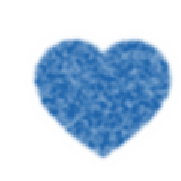
\includegraphics[width=.17\linewidth]{figures/monge-shape-mccann-interpolation--density-t100.pdf} \\[-.1em]
\small $t=0$ & \small $t=1/4$ & \small $t=1/2$ & \small $t=3/4$ & \small $t=1$
\end{tabular}
\caption{McCann displacement interpolation between a cat silhouette and a heart silhouette. The first row displays a small farthest-point subset of transported particles along $T_t(x)=(1-t)x+tT(x)$. The second row renders kernel-smoothed densities from a denser transported cloud as color images: white means zero density, while high density saturates in the red-to-blue interpolation color of the corresponding time.}
\index{displacement!interpolation}% strictindex
\label{fig:monge-shape-mccann-interpolation}
\end{figure}

Caffarelli's regularity theory, discussed next, explains when the convex potential is actually smooth enough to define a classical deformation.
\index{regularity theory}% strictindex
\index{Caffarelli regularity}% strictindex
\index{convex!potential}% strictindex

\paragraph{Regularity and the Monge--Amp\`ere equation.}
\index{Monge-Ampere equation}% strictindex

The previous results identify the optimal map; regularity theory asks when this map is a classical smooth deformation rather than only an almost-everywhere gradient. For quadratic costs this question becomes the regularity theory of the Monge--Amp\`ere equation.
\index{regularity theory}% strictindex
\index{Monge-Ampere equation}% strictindex
\index{cost!quadratic}% strictindex

\begin{prop}[Caffarelli regularity]\label{prop-caffarelli-regularity}
\index{Caffarelli regularity}% strictindex
	Let $\Omega,\Lambda\subset\RR^d$ be bounded uniformly convex domains with $C^2$ boundaries. Let $\al=\rho(x)\d x$ be supported on $\Omega$ and $\be=\eta(y)\d y$ be supported on $\Lambda$, with $0<m\leq\rho,\eta\leq M<+\infty$. If $\rho,\eta\in C^\alpha$ for some $\alpha\in(0,1)$, then the Brenier potential $\phi$ transporting $\al$ to $\be$ is strictly convex and satisfies $\phi\in C^{2,\alpha}_{\mathrm{loc}}(\Omega)$; in particular $\nabla\phi$ is locally H\"older. Under the corresponding boundary compatibility and smoothness assumptions, the regularity holds up to the boundary.
\end{prop}
\begin{proof}
	The potential solves the Monge--Amp\`ere equation
\index{Monge-Ampere equation}% strictindex
	\[
		\det(\nabla^2\phi(x))
		=
		\frac{\rho(x)}{\eta(\nabla\phi(x))}
	\]
	in the Alexandrov sense, with second boundary condition $\nabla\phi(\Omega)=\Lambda$. The density bounds and convexity of the domains give strict convexity and localization of sections. Caffarelli's interior theory then yields $C^{2,\alpha}_{\mathrm{loc}}$ estimates for $\phi$; the boundary statement follows from the boundary regularity theory under uniform convexity and compatibility assumptions~\cite{caffarelli2003monge,Villani09}.
\index{second boundary condition}% strictindex
\index{localization}% strictindex
\index{regularity theory}% strictindex
\index{Alexandrov solution}% strictindex
\index{strict!convexity}% strictindex
\end{proof}

\begin{rem}[Regularity, weak maps, and splitting]
\index{weak!map}% strictindex
\index{splitting obstruction}% strictindex
	Caffarelli's theorem should be read as a warning as well as a theorem. Brenier's theorem gives existence and uniqueness under mild assumptions, but smoothness requires density bounds, smoothness and convex geometry that are rarely satisfied by empirical, manifold-supported or neural generative distributions. In such applications, the exact OT map is often only weakly defined, possibly unstable, and better represented by a coupling, an entropic approximation or a learned parametric surrogate.
\index{exact OT}% strictindex
\index{Brenier!theorem}% strictindex

	Even without smoothness, the convex potential is locally Lipschitz on the interior of its domain, so $\nabla\phi$ is defined Lebesgue-almost everywhere. If the source measure does not satisfy the non-splitting hypotheses of Brenier's theorem, the correct relaxed object is instead an optimal Kantorovich plan concentrated on the graph of the set-valued map $\partial\phi$. At points where $\partial\phi(x)$ contains several target locations, the plan may split the mass starting from $x$. Thus the subdifferential still describes the geometry of optimality, but the transport object is a coupling rather than a single-valued map.
\index{subdifferential}% strictindex
\index{convex!potential}% strictindex
\end{rem}

For smooth densities, the change-of-variables formula~\eqref{eq-pfwd-density} gives the Monge--Amp\`ere equation
\index{change-of-variables}% strictindex
\index{change-of-variables formula}% strictindex
\index{Monge-Ampere equation}% strictindex
\eql{\label{eq-monge-ampere}
	\det(\nabla^2\phi(x))\density{\be}(\nabla\phi(x))=\density{\al}(x).
}
With suitable boundary conditions, this characterizes the Brenier potential up to an additive constant among convex solutions. The convexity constraint forces $\det(\nabla^2\phi(x))\geq0$ and is necessary for this fully nonlinear elliptic equation to be well posed. Numerical schemes for this PDE connect OT with fully nonlinear elliptic solvers; see for instance~\cite{Benamou:2014jw,froese2011convergent}.

The following proposition records the infinitesimal form of this nonlinear equation. It is useful both conceptually and numerically: close to a smooth reference density, Monge--Amp\`ere transport reduces at first order to a weighted Poisson equation.
\index{weighted!Poisson equation}% strictindex

\begin{prop}[Linearization of the Monge--Amp\`ere equation]\label{prop-linearized-monge-ampere}
\index{Monge-Ampere equation}% strictindex
\index{linear!linearization}% strictindex
	Let $\rho_\epsilon=\rho_0+\epsilon r+o(\epsilon)$ be a smooth perturbation of a positive reference density $\rho_0$ on a smooth bounded domain, with $\int r=0$. If $\T_\epsilon(x)=x+\epsilon\nabla u(x)+o(\epsilon)$ transports $\rho_0$ to $\rho_\epsilon$, then, to first order,
	\[
		-\nabla\cdot(\rho_0\nabla u)=r.
	\]
	In particular, when $\rho_0$ is constant, the linearized equation is $-\Delta u=r/\rho_0$.
\end{prop}
\begin{proof}
	The change-of-variables equation for $\T_\epsilon$ is
\index{change-of-variables}% strictindex
	\[
		\rho_0(x)
		=
		\rho_\epsilon(\T_\epsilon(x))\det(\nabla \T_\epsilon(x)).
	\]
	Expanding $\rho_\epsilon(x+\epsilon\nabla u)=\rho_0(x)+\epsilon r(x)+\epsilon\dotp{\nabla\rho_0}{\nabla u}+o(\epsilon)$ and
	\[
		\det(I+\epsilon\nabla^2u)=1+\epsilon\Delta u+o(\epsilon)
	\]
	gives
	\[
		\rho_0
		=
		\rho_0+
		\epsilon\bigl(r+\dotp{\nabla\rho_0}{\nabla u}+\rho_0\Delta u\bigr)+o(\epsilon)
		=
		\rho_0+
		\epsilon\bigl(r+\nabla\cdot(\rho_0\nabla u)\bigr)+o(\epsilon).
	\]
	The first-order term must vanish.
\end{proof}

%%%%%%%%%%%%%%%%%%%%%%%%%%%%%%%%%%%%%%%%%%%%%%%%%%%%%%%%%%%%%%%%%%%%%%%%%%%
\section{One-Dimensional Transport and Quantiles}
\index{one-dimensional!transport}% strictindex
\index{quantile}% strictindex
\label{sec-1d-transport-quantiles}

In one dimension, optimal transport is completely explicit. The cumulative distribution function orders the mass, and the optimal coupling is obtained by matching equal quantile levels. This special case is both a computational tool and the template for several linearized constructions used later.
\index{optimal coupling}% strictindex
\index{cumulative!distribution function}% strictindex

\begin{defn}[Cumulative and quantile functions]\label{def-cdf-quantile}
\index{cumulative!function}% strictindex
\index{quantile!function}% strictindex
	For $\al\in\Mm_+^1(\RR)$, its cumulative distribution function is
	\eql{\label{eq-cumul-defn}
		\cumul{\al}(x)\eqdef\al((-\infty,x]).
	}
	Its generalized inverse, or quantile function, is
\index{generalized!inverse}% strictindex
\index{quantile!function}% strictindex
	\eql{\label{eq-OT-map-1d}
		\cumul{\al}^{-1}(r)
		\eqdef
		\inf\enscond{x\in\RR}{\cumul{\al}(x)\geq r},
		\qquad r\in(0,1).
	}
\end{defn}

\begin{prop}[Quantile push-forward]\label{prop-quantile-pushforward}
\index{push-forward}% strictindex
\index{quantile!push-forward}% strictindex
	One has $(\cumul{\al}^{-1})_\sharp\mathrm{Leb}_{[0,1]}=\al$. If $\al$ has no atoms, then $(\cumul{\al})_\sharp\al=\mathrm{Leb}_{[0,1]}$.
\end{prop}
\begin{proof}
	For simplicity, assume first that $\al$ has a strictly positive density, so that $\cumul{\al}$ is strictly increasing and continuous. Denote $\ga\eqdef(\cumul{\al}^{-1})_\sharp\mathrm{Leb}_{[0,1]}$. It is enough to prove that $\cumul{\ga}=\cumul{\al}$. For every $x$,
	\[
	\begin{aligned}
		\cumul{\ga}(x)
		&=
		\int_0^1 \mathbf 1_{(-\infty,x]}(\cumul{\al}^{-1}(z))\d z
		=
		\int_0^1 \mathbf 1_{[0,\cumul{\al}(x)]}(z)\d z
		=
		\cumul{\al}(x),
	\end{aligned}
	\]
	where we used $\cumul{\al}^{-1}(z)\leq x$ if and only if $z\leq\cumul{\al}(x)$. General measures follow from the same argument with generalized inverses and right-continuity of the cumulative distribution function. If $\al$ has no atoms, the probability integral transform gives $(\cumul{\al})_\sharp\al=\mathrm{Leb}_{[0,1]}$.
\index{cumulative!distribution function}% strictindex
\index{generalized!inverse}% strictindex
\end{proof}

If $\al$ has no atoms, the map
\eql{\label{eq-1d-monge-map}
	\T=\cumul{\be}^{-1}\circ\cumul{\al}
}
satisfies $\T_\sharp\al=\be$.

For the cost $c(x,y)=|x-y|^2$, this map is nondecreasing, hence the derivative of a convex function in dimension one. Brenier's theorem therefore identifies it as the optimal Monge map whenever $\al$ is atomless. With generalized inverses, the same quantile construction gives the optimal Kantorovich coupling for arbitrary measures, and it is also optimal for costs of the form $h(|x-y|)$ with $h$ convex and nondecreasing.
\index{Monge!problem}% strictindex
\index{convex!function}% strictindex
\index{Brenier!theorem}% strictindex
\index{generalized!inverse}% strictindex

\begin{prop}[Monotone rearrangement on the line]\label{prop-1d-quantile-map}
\index{monotone!rearrangement}% strictindex
\index{quantile!map}% strictindex
	Let $\al,\be\in\Mm_+^1(\RR)$ have finite $p$-th moments, with $p\geq1$. The coupling
	\[
		\pi^\star=(\cumul{\al}^{-1},\cumul{\be}^{-1})_\sharp\mathrm{Leb}_{[0,1]}
	\]
	minimizes $\int |x-y|^p\d\pi(x,y)$ among couplings. If $\al$ has no atoms, it is induced by the monotone Monge map~\eqref{eq-1d-monge-map}.
\index{Monge!problem}% strictindex
\end{prop}
\begin{proof}
		The displayed measure is a coupling by Proposition~\ref{prop-quantile-pushforward}. Its support is monotone: for $s<t$, both quantile functions satisfy $\cumul{\al}^{-1}(s)\leq\cumul{\al}^{-1}(t)$ and $\cumul{\be}^{-1}(s)\leq\cumul{\be}^{-1}(t)$. If a coupling had two crossed pairs $x<x'$ and $y>y'$ with positive mass, exchanging the targets decreases the cost for strictly convex powers and does not increase it for $p=1$, by the two-point inequality used in Proposition~\ref{prop-matching-1d-monotone}. Eliminating crossings yields a monotone optimal coupling, and the monotone coupling with prescribed marginals is exactly the quantile coupling. If $\al$ has no atoms, $(\cumul{\al})_\sharp\al=\mathrm{Leb}_{[0,1]}$, so the coupling is generated by~\eqref{eq-1d-monge-map}.
\index{optimal coupling}% strictindex
\index{push-forward}% strictindex
\index{quantile!function}% strictindex
\end{proof}

\begin{rem}[Composition is one-dimensional]\label{rem-1d-composition-optimal}
	In dimension one, optimal maps compose. Assume for simplicity that the intermediate laws have no atoms, so that the monotone rearrangements
\index{monotone!rearrangement}% strictindex
	\[
		\T_{\al\to\be}=\cumul{\be}^{-1}\circ\cumul{\al},
		\qquad
		\T_{\be\to\ga}=\cumul{\ga}^{-1}\circ\cumul{\be}
	\]
	are well defined $\al$- and $\be$-almost everywhere. Then
	\[
		\T_{\be\to\ga}\circ\T_{\al\to\be}
		=
		\T_{\al\to\ga}
		\qquad \al\text{-a.e.}
	\]
	Indeed, each map is nondecreasing and sends quantile level $r$ to the same quantile level of the target law. This semigroup property is special to the ordered line.
\end{rem}

The obstruction in higher dimension is already visible for the most elementary Gaussian maps.

\begin{example}[Linear obstruction to composing Brenier maps]
	In higher dimension, Brenier maps for the quadratic cost are gradients of convex functions, and such maps do not generally remain gradients after composition. The simplest obstruction is linear. If $\T_1(x)=A_1x$ and $\T_2(x)=A_2x$ with $A_1,A_2$ symmetric positive definite, then $\T_2\circ\T_1$ has matrix $A_2A_1$. It is a gradient field only when this product is symmetric, equivalently $A_1A_2=A_2A_1$. Gaussian transport gives a concrete instance: between nondegenerate Gaussian laws, the Brenier map is affine with symmetric positive definite linear part. Compositions of Gaussian optimal maps are therefore optimal only in special commuting situations, for instance when all covariance matrices are simultaneously diagonalizable. Otherwise the composition contains a rotational or shearing component and is not the Brenier map between the initial and final Gaussians.
\index{rotational component}% strictindex
\index{shearing component}% strictindex
\index{convex!function}% strictindex
\index{covariance!matrix}% strictindex
\index{Gaussian!optimal map}% strictindex
\index{cost!quadratic}% strictindex
\index{Brenier!map}% strictindex
\end{example}

For discrete measures, one cannot directly apply the map formula when the source has atoms, but if the measures are uniform on the same number of Dirac masses, then it is exactly the sorting formula of Proposition~\ref{prop-matching-1d-monotone}.
\index{Dirac mass}% strictindex

\begin{alg}[Quantile rearrangement and one-dimensional geodesic]\label{alg:quantile-rearrangement-geodesic}
\index{quantile!map}% strictindex
\index{one-dimensional!transport}% strictindex
\textbf{Input:} One-dimensional probability measures $\alpha,\beta$; time $t\in[0,1]$.

\textbf{Output:} Quantile coupling, Monge map when defined, and geodesic point $\alpha_t$.

\textbf{Compute} $\cumul{\al}$, $\cumul{\be}$ and generalized inverses.

\textbf{Couple} equal quantile levels:
\(X=\cumul{\al}^{-1}(r), \qquad Y=\cumul{\be}^{-1}(r), \qquad r\in(0,1).\)

\textbf{If} $\alpha$ has no atoms \textbf{then}:
\begin{algblock}

\textbf{Set}
\(T(x)=\cumul{\be}^{-1}(\cumul{\al}(x)).\)
\end{algblock}
\textbf{Interpolate} quantiles:
\(Q_t(r)=(1-t)\cumul{\al}^{-1}(r)+t\cumul{\be}^{-1}(r), \qquad \al_t=(Q_t)_\sharp\mathrm{Leb}_{[0,1]}.\)
\textbf{Return} $(X,Y)$, $T$ if defined, and $\alpha_t$.
\end{alg}

\begin{prop}[One-dimensional Wasserstein formulas]\label{prop-wass-quantile-1d}
\index{Wasserstein!formula}% strictindex
	Let $\al,\be\in\Mm_+^1(\RR)$ have finite $p$-th moments. For every $p\geq1$,
	\eql{\label{eq-wass-cumul}
		\Wass_p(\al,\be)^p
		=
		\int_0^1\abs{\cumul{\al}^{-1}(r)-\cumul{\be}^{-1}(r)}^p\d r
		=
		\norm{\cumul{\al}^{-1}-\cumul{\be}^{-1}}_{L^p([0,1])}^p.
	}
	For $p=1$, this is equivalently
	\begin{align}\label{eq-w1-1d}
		\Wass_1(\al,\be)
		&=
		\norm{\cumul{\al}-\cumul{\be}}_{L^1(\RR)}
		=
		\int_\RR \abs{\cumul{\al}(x)-\cumul{\be}(x)}\d x \\
		&=
		\int_\RR \abs{\int_{-\infty}^x\d(\al-\be)}\d x.
	\end{align}
\end{prop}
\begin{proof}
	The first formula follows from Proposition~\ref{prop-1d-quantile-map}: the optimal coupling is obtained by taking the same quantile level $r$ for both measures. For $p=1$, use the layer-cake identity. If $q_\al$ and $q_\be$ are the two quantile functions, then
\index{optimal coupling}% strictindex
\index{quantile!function}% strictindex
\index{quantile!map}% strictindex
	\[
		\int_0^1 |q_\al(r)-q_\be(r)|\d r
		=
		\int_\RR
		\lambda\bigl(\{r:q_\al(r)\leq x<q_\be(r)\}\cup\{r:q_\be(r)\leq x<q_\al(r)\}\bigr)\d x.
	\]
	The measure of the displayed set is exactly $|\cumul{\al}(x)-\cumul{\be}(x)|$ for almost every $x$.
\end{proof}

Formula~\eqref{eq-wass-cumul} means that the map $\al\mapsto\cumul{\al}^{-1}$ embeds one-dimensional Wasserstein geometry isometrically into a linear $L^p$ space. For $p=2$, the Wasserstein distance on probability measures over the real line is therefore Hilbertian. This makes one-dimensional OT much simpler than higher-dimensional OT, where the Wasserstein geometry is not globally Hilbertian.
\index{probability measure}% strictindex
\index{Wasserstein!distance}% strictindex

\begin{figure}[htbp]
\centering
\setlength{\tabcolsep}{2pt}
\begin{tabular}{@{}cccc@{}}
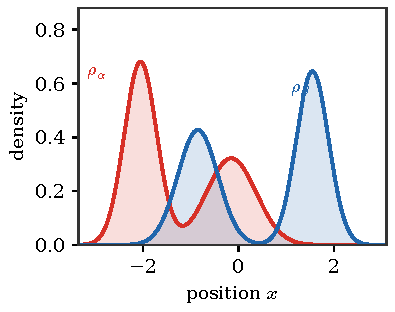
\includegraphics[width=.24\linewidth]{figures/monge-1d-quantile-geodesic--endpoint-densities.pdf} &
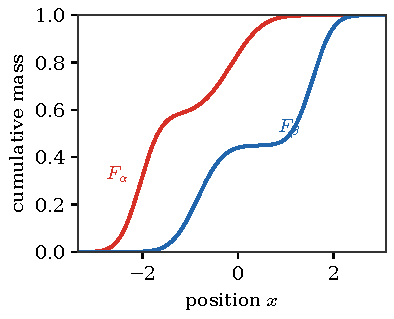
\includegraphics[width=.24\linewidth]{figures/monge-1d-quantile-geodesic--cdfs.pdf} &
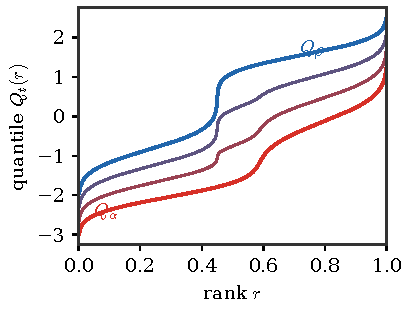
\includegraphics[width=.24\linewidth]{figures/monge-1d-quantile-geodesic--quantiles.pdf} &
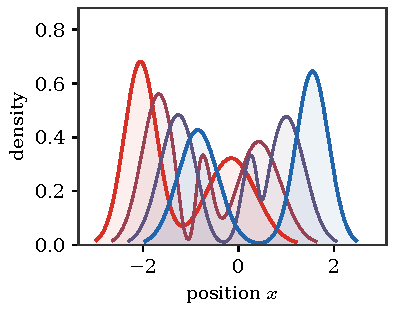
\includegraphics[width=.24\linewidth]{figures/monge-1d-quantile-geodesic--geodesic-densities.pdf} \\[-.1em]
\small densities &
\small cumulative functions &
\small quantiles &
\small displacement geodesic
\end{tabular}
\caption{One-dimensional transport through quantiles. The same two smooth laws are shown as densities, cumulative functions and quantile functions. The last panel displays the displacement interpolation obtained by the linear quantile path $Q_t=(1-t)Q_\alpha+tQ_\beta$, which is the explicit one-dimensional $\Wass_2$ geodesic.}
\index{one-dimensional!transport}% strictindex
\index{displacement!interpolation}% strictindex
\index{quantile!function}% strictindex
\label{fig:monge-1d-quantile-geodesic}
\end{figure}

The last panel of Figure~\ref{fig:monge-1d-quantile-geodesic} is the one-dimensional specialization of the displacement interpolation of Section~\ref{sec-monge-interpolation}. In quantile coordinates, the interpolating measure is characterized by
\index{displacement!interpolation}% strictindex
\index{Monge!interpolation}% strictindex
\[
	\cumul{\al_t}^{-1}(r)
	=
	(1-t)\cumul{\al}^{-1}(r)+t\cumul{\be}^{-1}(r),
	\qquad r\in(0,1).
\]
The histogram-equalization figure in Section~\ref{sec-monge-pbm} is the same construction applied to pixel intensities.
\index{histogram}% strictindex

For $p=1$, formula~\eqref{eq-w1-1d} shows that $\Wass_1$ is a norm on signed measures with zero total mass once they are identified with their cumulative primitives. Other classical one-dimensional distances are obtained by replacing the $L^1$ norm of cumulative functions with $L^2$ or $L^\infty$ norms; under suitable tightness assumptions, such norms also metrize convergence in law and lead for instance to Cram\'er--von Mises and Kolmogorov--Smirnov-type distances.
\index{convergence!in law}% strictindex
\index{Cramer-von Mises distance}% strictindex
\index{Kolmogorov-Smirnov distance}% strictindex
\index{tightness}% strictindex
\index{cumulative!function}% strictindex
\index{signed!measure}% strictindex

\paragraph{Triangular rearrangements.}
\index{triangular!rearrangement}% strictindex

There is another canonical way to build transport maps in several dimensions: transport one coordinate at a time by conditional one-dimensional quantiles. This construction goes back to Knothe and Rosenblatt~\cite{Knothe1957,Rosenblatt1952}. It is not usually cost-optimal, but it gives a deterministic rearrangement under weak assumptions and clarifies how multivariate transport can be reduced recursively to scalar monotone maps.
\index{transport map}% strictindex

\begin{prop}[Knothe--Rosenblatt triangular rearrangement]\label{prop-knothe-rosenblatt}
\index{Knothe-Rosenblatt rearrangement}% strictindex
	Let $\al,\be\in\Mm_+^1(\RR^d)$. Assume, for simplicity, that the first marginal of $\al$ and the one-dimensional conditional laws of $\al$ used below are atomless, and that regular conditional distributions are fixed. There is a triangular map
\index{regular conditional distribution}% strictindex
\index{conditional law}% strictindex
\index{triangular!map}% strictindex
	\[
		\T(x_1,\ldots,x_d)
		=
		(\T_1(x_1),\T_2(x_1,x_2),\ldots,\T_d(x_1,\ldots,x_d))
	\]
	such that $\T_\sharp\al=\be$ and, for each $k$, the function $x_k\mapsto\T_k(x_1,\ldots,x_k)$ is nondecreasing for $\al$-almost every value of $(x_1,\ldots,x_{k-1})$.
\end{prop}
\begin{proof}
	The construction is recursive. For $k=1$, let $\T_1$ be the monotone rearrangement between the first marginal of $\al$ and the first marginal of $\be$. Suppose that $\T_1,\ldots,\T_{k-1}$ have already been constructed. Write $x_{<k}=(x_1,\ldots,x_{k-1})$ and $\T_{<k}=(\T_1,\ldots,\T_{k-1})$. By induction, $(\T_{<k})_\sharp\al_{<k}=\be_{<k}$, where $\al_{<k}$ and $\be_{<k}$ are the first $(k-1)$-coordinate marginals. Let $\al^k_{x_{<k}}$ and $\be^k_{y_{<k}}$ be regular conditional laws of the $k$-th coordinate given the previous coordinates. Define $\T_k(x_{<k},\cdot)$ as the one-dimensional monotone rearrangement from $\al^k_{x_{<k}}$ to $\be^k_{\T_{<k}(x_{<k})}$.
\index{monotone!rearrangement}% strictindex

	The map $\T_k(x_{<k},\cdot)$ is nondecreasing by the one-dimensional rearrangement theorem. The chain rule for disintegrations then shows that, after step $k$, the first $k$ coordinates of $\T_\sharp\al$ have the same law as the first $k$ coordinates of $\be$. At $k=d$ this gives $\T_\sharp\al=\be$. Target atoms are handled by generalized quantiles. If a source conditional law has atoms that must be split, the same recursive construction defines a triangular Markov kernel rather than a deterministic map.
\index{disintegration}% strictindex
\index{Markov kernel}% strictindex
\index{generalized quantile}% strictindex
\index{conditional law}% strictindex
\end{proof}

The recursive construction in the proof is an algorithm: it repeatedly applies the one-dimensional quantile rearrangement to conditional distributions.

\begin{alg}[Knothe--Rosenblatt triangular rearrangement]\label{alg:triangular-rearrangement}
\textbf{Input:} Probability measures $\alpha,\beta$ on $\RR^d$ with conditional laws.

\textbf{Output:} Knothe--Rosenblatt triangular map $\T$.

\textbf{Compute} first-coordinate rearrangement:
\(\T_1=(F_{\be_1})^{-1}\circ F_{\al_1}.\)

\textbf{For} $k=2,\ldots,d$ \textbf{do}:
\begin{algblock}

\textbf{Set} $x_{<k}=(x_1,\ldots,x_{k-1})$.

\textbf{Compute} conditional laws $\al^k_{x_{<k}}$ and $\be^k_{\T_{<k}(x_{<k})}$.

\textbf{Set}
\(\T_k(x_{<k},x_k) = \bigl(F_{\be^k_{\T_{<k}(x_{<k})}}\bigr)^{-1} \circ F_{\al^k_{x_{<k}}}(x_k).\)
\end{algblock}
\algreturnskip
\textbf{Return} \(\T(x)=(\T_1(x_1),\T_2(x_1,x_2),\ldots,\T_d(x_1,\ldots,x_d)).\)
\end{alg}

Figure~\ref{fig:monge-triangular-rearrangement} shows the two-dimensional mechanism on image histograms. The first stage transports only the horizontal marginal, so the middle pivot has the same $x$-marginal as the target but keeps the source vertical conditionals. The second stage then transports each vertical conditional law inside the corresponding column.
\index{histogram}% strictindex
\index{conditional law}% strictindex
\index{triangular!rearrangement}% strictindex

\begin{figure}[H]
\centering
\setlength{\tabcolsep}{1pt}
\begin{tabular}{@{}ccccccc@{}}
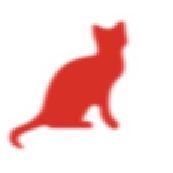
\includegraphics[width=.135\linewidth]{figures/monge-triangular-rearrangement--stage-01-source.pdf} &
\index{triangular!rearrangement}% strictindex

\includegraphics[width=.135\linewidth]{figures/monge-triangular-rearrangement--stage-02-horizontal-033.pdf} &
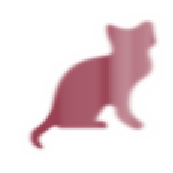
\includegraphics[width=.135\linewidth]{figures/monge-triangular-rearrangement--stage-03-horizontal-067.pdf} &
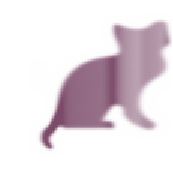
\includegraphics[width=.135\linewidth]{figures/monge-triangular-rearrangement--stage-04-pivot.pdf} &
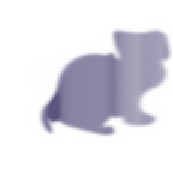
\includegraphics[width=.135\linewidth]{figures/monge-triangular-rearrangement--stage-05-vertical-033.pdf} &
\index{triangular!rearrangement}% strictindex
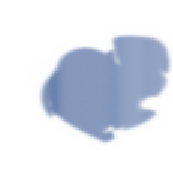
\includegraphics[width=.135\linewidth]{figures/monge-triangular-rearrangement--stage-06-vertical-067.pdf} &

\includegraphics[width=.135\linewidth]{figures/monge-triangular-rearrangement--stage-07-target.pdf} \\[-.1em]
\small source &
\small $x$-move &
\small $x$-move &
\small pivot &
\small $y$-move &
\small $y$-move &
\small target
\end{tabular}
\caption{Triangular rearrangement between the same cat and heart densities as in Figure~\ref{fig:monge-shape-mccann-interpolation}. The panels are computed directly on image histograms. The first three transitions move mass horizontally by the monotone rearrangement between the $x$-marginals; the pivot has the target horizontal marginal. The last three transitions keep each column fixed and move mass vertically by one-dimensional monotone rearrangements between conditional laws.}
\index{triangular!rearrangement}% strictindex
\index{monotone!rearrangement}% strictindex
\index{McCann interpolation}% strictindex
\label{fig:monge-triangular-rearrangement}
\end{figure}

This construction transports successively along coordinate axes and is therefore often called axis-wise transport. It depends on the chosen ordering of coordinates and is not generally optimal for the quadratic cost. It is nevertheless a useful limiting object: Brenier maps for increasingly anisotropic quadratic costs converge to triangular rearrangements under suitable assumptions~\cite{carlier2010knothe}.
\index{triangular!rearrangement}% strictindex
\index{cost!quadratic}% strictindex
\index{Brenier!map}% strictindex

\begin{prop}[Anisotropic Brenier maps converge to Knothe--Rosenblatt]\label{prop-knothe-limit-anisotropic-brenier}
\index{Knothe-Rosenblatt rearrangement}% strictindex
	Let $\alpha,\beta$ be compactly supported probability measures on $\RR^d$ with densities bounded above and below on their rectangular supports, and assume that the conditional laws entering Proposition~\ref{prop-knothe-rosenblatt} are atomless. For $\epsilon>0$, set
\index{conditional law}% strictindex
\index{probability measure}% strictindex
	\[
		c_\epsilon(x,y)
		\eqdef
		\sum_{k=1}^d \epsilon^{k-1}\abs{x_k-y_k}^2 .
	\]
	Let $T_\epsilon$ be the Monge map from $\alpha$ to $\beta$ for the cost $c_\epsilon$, and let $T_{\mathrm{KR}}$ be the triangular Knothe--Rosenblatt rearrangement with the coordinate order used above. Then
\index{Monge!problem}% strictindex
\index{Knothe-Rosenblatt rearrangement}% strictindex
	\[
		T_\epsilon \longrightarrow T_{\mathrm{KR}}
		\qquad\text{in } L^2(\alpha;\RR^d)
		\qquad\text{as } \epsilon\to0 .
	\]
\end{prop}

\begin{proof}
	We give the standard lexicographic argument, which is the variational core of~\cite{carlier2010knothe}. Let $\pi_\epsilon=(\Id,T_\epsilon)_\sharp\alpha$. Since the supports are compact, a subsequence converges weakly to some coupling $\pi$ between $\alpha$ and $\beta$. The optimality of $\pi_\epsilon$ for
	\[
		F_\epsilon(\gamma)
		=
		\sum_{k=1}^d \epsilon^{k-1}
		\int\abs{x_k-y_k}^2\d\gamma(x,y)
	\]
	first implies, by letting $\epsilon\to0$, that $\pi$ minimizes the one-dimensional quadratic cost in the first coordinate among all couplings. Since the first marginal of $\alpha$ is atomless, the one-dimensional minimizer is the monotone rearrangement, so $y_1=T_1(x_1)$ under $\pi$.
\index{monotone!rearrangement}% strictindex
\index{cost!quadratic}% strictindex

	Now restrict attention to couplings satisfying this first-coordinate constraint. Subtract the common minimal value of the first-coordinate cost, divide the optimality inequality by $\epsilon$, and let $\epsilon\to0$. The limit coupling must minimize the second-coordinate quadratic cost among all couplings that already realize the first monotone rearrangement. Disintegrating with respect to $(x_1,y_1)$ reduces this constrained problem to the one-dimensional monotone rearrangement between the conditional laws of $x_2$ and $y_2$. Hence $y_2=T_2(x_1,x_2)$ under $\pi$.
\index{conditional law}% strictindex

	Repeating the same subtraction-and-rescaling argument gives, for every $k$, the conditional monotone rearrangement $y_k=T_k(x_1,\ldots,x_k)$. Thus every weak limit of $(\pi_\epsilon)_\epsilon$ is concentrated on the graph of $T_{\mathrm{KR}}$. This graph coupling is unique, so the whole family $\pi_\epsilon$ converges weakly to $(\Id,T_{\mathrm{KR}})_\sharp\alpha$.
\index{weak!limit}% strictindex
\index{monotone!rearrangement}% strictindex

	Finally, let $X\sim\alpha$. The graph couplings are the laws of $(X,T_\epsilon(X))$, and they converge weakly to the law of $(X,T_{\mathrm{KR}}(X))$. To turn this into convergence of maps, fix $\zeta>0$. By Lusin's theorem, there is a compact set $K$ with $\alpha(K)>1-\zeta$ on which $T_{\mathrm{KR}}$ is continuous. On $K$, the set
	\[
		\enscond{(x,y)}{x\in K,\ \norm{y-T_{\mathrm{KR}}(x)}\geq\delta}
	\]
	is closed and has zero mass under the limiting graph coupling. Portmanteau's theorem gives
\index{zero mass}% strictindex
	\[
		\limsup_{\epsilon\to0}
		\alpha\!\left(\enscond{x}{x\in K,\ \norm{T_\epsilon(x)-T_{\mathrm{KR}}(x)}\geq\delta}\right)
		=0 .
	\]
	Adding the complement of $K$ and letting $\zeta\to0$ proves convergence in $\alpha$-probability. Since all maps take values in a common compact set, this convergence is uniformly integrable and hence holds in $L^2(\alpha)$.
\end{proof}

%%%%%%%%%%%%%%%%%%%%%%%%%%%%%%%%%%%%%%%%%%%%%%%%%%%%%%%%%%%%%%%%%%%%%%%%%%%
\section{Gaussian Measures and the Bures Metric}
\index{Gaussian!measure}% strictindex
\index{Bures!metric}% strictindex
\label{sec-gaussian-bures}

Gaussian measures form the most important finite-dimensional family preserved by quadratic optimal transport. The mean moves linearly, while the covariance follows the Bures--Wasserstein geometry of positive semidefinite matrices.
\index{positive!semidefinite matrix}% strictindex
\index{Bures-Wasserstein geometry}% strictindex

\paragraph{One-dimensional Gaussians.}
\index{Gaussian!measure}% strictindex

Let $\al=\Gaussian(m_\al,\sigma_\al^2)$ and $\be=\Gaussian(m_\be,\sigma_\be^2)$ be two nondegenerate Gaussians on $\RR$. Then
\[
	\T(x)=\frac{\sigma_\be}{\sigma_\al}(x-m_\al)+m_\be
\]
satisfies $\T_\sharp\al=\be$. It is the derivative of the convex function
\index{convex!function}% strictindex
\[
	\phi(x)=\frac{\sigma_\be}{2\sigma_\al}(x-m_\al)^2+m_\be x,
\]
so Brenier's theorem shows that it is the optimal quadratic transport. The associated distance is
\index{Brenier!theorem}% strictindex
\[
	\Wass_2(\al,\be)^2
	=
	\int_\RR\left(\frac{\sigma_\be}{\sigma_\al}(x-m_\al)+m_\be-x\right)^2\d\al(x)
	=
	(m_\al-m_\be)^2+(\sigma_\al-\sigma_\be)^2.
\]
The formula extends by continuity to Dirac masses, although the affine Monge map itself only pushes a Dirac source to another Dirac. Thus the OT geometry of one-dimensional Gaussians is the Euclidean geometry of the half-plane $(m,\sigma)\in\RR\times\RR_+$. This contrasts with KL geometry, where singular Gaussians are infinitely distant.
\index{Monge!problem}% strictindex
\index{Dirac mass}% strictindex
\index{Gaussian!measure}% strictindex

\begin{figure}[htbp]
\centering
\setlength{\tabcolsep}{2pt}
\begin{tabular}{@{}ccc@{}}
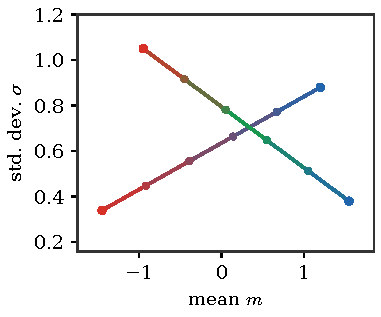
\includegraphics[width=.30\linewidth]{figures/monge-gaussian-w2-geodesic--halfplane-1d.pdf} &
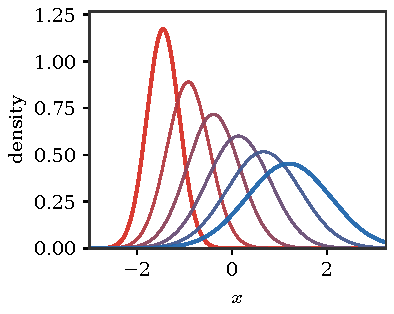
\includegraphics[width=.32\linewidth]{figures/monge-gaussian-w2-geodesic--densities-1d-a.pdf} &
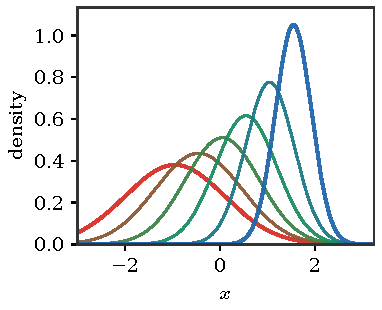
\includegraphics[width=.32\linewidth]{figures/monge-gaussian-w2-geodesic--densities-1d-b.pdf} \\[-.1em]
\small $(m,\sigma)$ half-plane &
\small first geodesic &
\small second geodesic
\end{tabular}
\caption{One-dimensional Gaussian $\Wass_2$ geodesics. In the coordinates $(m,\sigma)$, the geodesics are Euclidean segments in the upper half-plane. The two density panels show the corresponding Gaussian densities along the two segments, with colors interpolating from the red endpoint to the blue endpoint.}
\label{fig:monge-gaussian-w2-geodesic-1d}
\end{figure}

\paragraph{Multivariate Gaussians.}
\index{Gaussian!measure}% strictindex

If
\eql{\label{eq-gauss-pf}
	\al=\Gaussian(\mean_\al,\cov_\al),
	\qquad
	\be=\Gaussian(\mean_\be,\cov_\be),
	\qquad
	\T(x)=\mean_\be+A(x-\mean_\al),
}
then $\T$ is the gradient of the convex quadratic potential $\phi(x)=\dotp{\mean_\be}{x}+\dotp{A(x-\mean_\al)}{x-\mean_\al}/2$ if and only if $A$ is symmetric positive semidefinite.
\index{quadratic!potential}% strictindex

\begin{prop}[Affine push-forward of Gaussians]\label{prop-gaussian-affine-push-forward}
\index{push-forward}% strictindex
\index{Gaussian!push-forward}% strictindex
	One has $\T_\sharp\al=\be$ if and only if
	\eql{\label{eq-gauss-covariance-pushforward}
		A\cov_\al A^\top=\cov_\be.
	}
\end{prop}
\begin{proof}
	An affine function maps a Gaussian to a Gaussian, so the law of $\T(X)$ is determined by its mean and covariance. If $X\sim\al$ and $Y=\T(X)$, then
	\[
		\EE(Y)=\mean_\be+A\EE(X-\mean_\al)=\mean_\be,
	\]
	and
	\[
		\EE((Y-\mean_\be)(Y-\mean_\be)^\top)
		=
		A\EE((X-\mean_\al)(X-\mean_\al)^\top)A^\top
		=
		A\cov_\al A^\top.
	\]
	Thus $A\cov_\al A^\top=\cov_\be$ is necessary and sufficient for $Y$ to have the same mean and covariance as $\be$.
\end{proof}

The covariance equation is quadratic in $A$. Under the symmetry constraint imposed by Brenier's theorem, it becomes $A\cov_\al A=\cov_\be$. The covariance part of the resulting cost is a matrix metric.
\index{Brenier!theorem}% strictindex

\begin{defn}[Bures metric]\label{def-bures-metric}
\index{Bures!metric}% strictindex
\index{positive!semidefinite matrix}% strictindex
	For positive semidefinite covariance matrices $\Sigma$ and $\Lambda$, the Bures metric is
	\eql{\label{eq-bure-defn}
		\Bb(\Sigma,\Lambda)^2
		\eqdef
		\tr\pa{\Sigma+\Lambda-2(\Sigma^{1/2}\Lambda\Sigma^{1/2})^{1/2}}.
	}
\end{defn}
The next proposition solves the covariance equation and shows that this metric is exactly the covariance contribution to Gaussian $\Wass_2$.

\begin{prop}[Gaussian $\Wass_2$ formula and Bures covariance term]\label{prop-gaussian-w2-bures}
\index{covariance!term}% strictindex
\index{Bures!covariance}% strictindex
	Assume that $\cov_\al$ and $\cov_\be$ are positive definite. The unique symmetric positive-definite solution of
	\[
		A\cov_\al A=\cov_\be
	\]
	is
	\eql{\label{eq-bures-map}
		A=
		\cov_\al^{-1/2}
		\pa{\cov_\al^{1/2}\cov_\be\cov_\al^{1/2}}^{1/2}
		\cov_\al^{-1/2}.
	}
	The affine map $\T(x)=\mean_\be+A(x-\mean_\al)$ is the optimal quadratic-cost transport from $\Gaussian(\mean_\al,\cov_\al)$ to $\Gaussian(\mean_\be,\cov_\be)$, and
\index{affine map}% strictindex
\index{cost!quadratic}% strictindex
	\eql{\label{eq-dist-gauss}
		\Wass_2(\al,\be)^2
		=
		\norm{\mean_\al-\mean_\be}^2+\Bb(\cov_\al,\cov_\be)^2,
	}
	where $\Bb$ is the Bures metric of Definition~\ref{def-bures-metric}.
\end{prop}
\begin{proof}
	Multiplying $A\cov_\al A=\cov_\be$ on the left and right by $\cov_\al^{1/2}$ gives
	\[
		(\cov_\al^{1/2}A\cov_\al^{1/2})^2
		=
		\cov_\al^{1/2}\cov_\be\cov_\al^{1/2}.
	\]
	Since $A$ is symmetric positive, $\cov_\al^{1/2}A\cov_\al^{1/2}$ is symmetric positive and is therefore the unique positive square root of the right-hand side. Conversely, the matrix in~\eqref{eq-bures-map} is symmetric positive and satisfies the covariance equation.

	By Proposition~\ref{prop-gaussian-affine-push-forward}, this affine map pushes $\al$ to $\be$. It is the gradient of a convex quadratic potential, so Brenier's theorem implies optimality. If $X\sim\al$, then
\index{affine map}% strictindex
\index{Brenier!theorem}% strictindex
\index{quadratic!potential}% strictindex
\index{push-forward}% strictindex
	\begin{align*}
		\EE\norm{X-\T(X)}^2
		&=
		\norm{\mean_\al-\mean_\be}^2
		+
		\EE\norm{(I-A)(X-\mean_\al)}^2 \\
		&=
		\norm{\mean_\al-\mean_\be}^2
		+
		\tr((I-A)\cov_\al(I-A)^\top) \\
		&=
		\norm{\mean_\al-\mean_\be}^2
		+
		\tr(\cov_\al)+\tr(A\cov_\al A)-2\tr(A\cov_\al) \\
		&=
		\norm{\mean_\al-\mean_\be}^2
		+
		\tr(\cov_\al)+\tr(\cov_\be)
		-2\tr((\cov_\al^{1/2}\cov_\be\cov_\al^{1/2})^{1/2}),
	\end{align*}
	which is the desired expression. The formula for singular covariance matrices follows by adding $\eta I$ and letting $\eta\downarrow0$.
\index{covariance!matrix}% strictindex
\end{proof}

The covariance term $\Bb$ is the Bures--Wasserstein metric on positive semidefinite matrices~\cite{bures1969extension,gelbrich1990formula,bhatia2018bures}. It separates the Euclidean displacement of the mean from the intrinsic transport geometry of covariance ellipsoids.
\index{Bures-Wasserstein geometry}% strictindex
\index{positive!semidefinite matrix}% strictindex
\index{covariance!term}% strictindex

\begin{figure}[htbp]
\centering
\setlength{\tabcolsep}{2pt}
\begin{tabular}{@{}cc@{}}
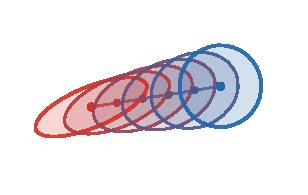
\includegraphics[width=.42\linewidth]{figures/monge-gaussian-w2-geodesic--ellipses-anisotropic-to-isotropic.pdf} &
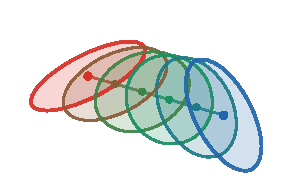
\includegraphics[width=.42\linewidth]{figures/monge-gaussian-w2-geodesic--ellipses-rotated-anisotropic.pdf} \\[-.1em]
\small anisotropic to isotropic &
\small rotated anisotropies
\end{tabular}
\caption{Two-dimensional Gaussian $\Wass_2$ geodesics. Means move linearly, while covariance ellipses follow the Bures--Wasserstein interpolation. The left panel contracts an anisotropic Gaussian toward an isotropic one; the right panel interpolates between two strongly oriented anisotropic covariances.}
\label{fig:monge-gaussian-w2-geodesic-2d}
\end{figure}

\begin{prop}[Metric and convexity properties of the Bures term]\label{prop-bures-metric-convex}
\index{Bures!metric}% strictindex
	The function $\Bb$ is a distance on positive semidefinite covariance matrices. Moreover, $\Bb^2$ is jointly convex: for $t\in[0,1]$,
\index{covariance!matrix}% strictindex
	\[
		\Bb^2((1-t)\Sigma_0+t\Sigma_1,(1-t)\Lambda_0+t\Lambda_1)
		\leq
		(1-t)\Bb^2(\Sigma_0,\Lambda_0)+t\Bb^2(\Sigma_1,\Lambda_1).
	\]
\end{prop}
\begin{proof}
	The key identity is the Procrustes representation
	\[
		\Bb^2(\Sigma,\Lambda)
		=
		\min_{Q^\top Q=I}\norm{\Sigma^{1/2}-\Lambda^{1/2}Q}_F^2.
	\]
	Indeed, expanding the square gives $\tr\Sigma+\tr\Lambda-2\max_{Q^\top Q=I}\tr(\Sigma^{1/2}Q^\top\Lambda^{1/2})$, and the orthogonal Procrustes formula identifies the maximum with $\tr((\Sigma^{1/2}\Lambda\Sigma^{1/2})^{1/2})$. Symmetry, positivity and separation follow immediately from this representation. The triangle inequality follows by choosing two almost optimal orthogonal matrices $Q_1,Q_2$ and writing
\index{triangle inequality}% strictindex
	\[
		\norm{\Sigma^{1/2}-\Gamma^{1/2}Q_2Q_1}_F
		\leq
		\norm{\Sigma^{1/2}-\Lambda^{1/2}Q_1}_F
		+
		\norm{\Lambda^{1/2}-\Gamma^{1/2}Q_2}_F.
	\]
	Letting the two choices become optimal proves the metric property.

	For convexity, use the equivalent factor formulation
	\[
		\Bb^2(\Sigma,\Lambda)
		=
		\min_{UU^\top=\Sigma,\thinspace VV^\top=\Lambda}\norm{U-V}_F^2.
	\]
	Choose nearly optimal factors $(U_0,V_0)$ and $(U_1,V_1)$ for the two pairs, and define block factors
	\[
		U_t=[\sqrt{1-t}\,U_0,\sqrt t\,U_1],
		\qquad
		V_t=[\sqrt{1-t}\,V_0,\sqrt t\,V_1].
	\]
	Then $U_tU_t^\top=(1-t)\Sigma_0+t\Sigma_1$ and $V_tV_t^\top=(1-t)\Lambda_0+t\Lambda_1$, while
	\[
		\norm{U_t-V_t}_F^2
		=
		(1-t)\norm{U_0-V_0}_F^2+t\norm{U_1-V_1}_F^2.
	\]
	Taking the infimum over the initial factors proves joint convexity.
\end{proof}

\begin{rem}[Diagonal covariances and Hellinger geometry]
\index{covariance!diagonal}% strictindex
\index{Hellinger!geometry}% strictindex
	If $\cov_\al=\diag(r_i)_i$ and $\cov_\be=\diag(s_i)_i$ are diagonal, the Bures metric reduces to the Euclidean distance between square roots,
\index{Bures!metric}% strictindex
	\[
		\Bb(\cov_\al,\cov_\be)=\norm{\sqrt r-\sqrt s}_2.
	\]
	This is the finite-dimensional Hellinger geometry on the nonnegative covariance coordinates: variances are compared after the amplitude change of variables $r_i\mapsto\sqrt{r_i}$.
\index{change-of-variables}% strictindex
\index{Hellinger!geometry}% strictindex
\end{rem}
